\documentclass[11pt,a4paper]{article}
\usepackage[utf8]{inputenc}
\usepackage[T1]{fontenc}
\usepackage{amsmath,amssymb,amsthm}
\usepackage{tikz}
\usetikzlibrary{arrows,arrows.meta,positioning,calc,shapes.geometric,decorations.markings}
\usepackage[margin=1cm,footskip=0.5cm]{geometry}
\usepackage[shortlabels]{enumitem}
\usepackage{hyperref}
\usepackage{tocloft}
\renewcommand{\cftsecfont}{\normalsize}
\renewcommand{\cftsubsecfont}{\normalsize}
\renewcommand{\cftsubsubsecfont}{\normalsize}
\renewcommand{\cftsecpagefont}{\normalsize}
\renewcommand{\cftsubsecpagefont}{\normalsize}
\renewcommand{\cftsubsubsecpagefont}{\normalsize}
\setcounter{tocdepth}{3}
\usepackage{titlesec}
\titleformat{\section}{\Large\bfseries}{\thesection}{0.5em}{}
\titleformat{\subsection}{\large\bfseries}{\thesubsection}{0.5em}{}
\titleformat{\subsubsection}{\normalsize\bfseries}{\thesubsubsection}{0.5em}{}
\renewcommand{\cftsecfont}{\large}
\renewcommand{\cftsubsecfont}{\normalsize}
\renewcommand{\cftsubsubsecfont}{\normalsize}
\renewcommand{\cftsecpagefont}{\large}
\renewcommand{\cftsubsecpagefont}{\normalsize}
\renewcommand{\cftsubsubsecpagefont}{\normalsize}
\usepackage{graphicx}
\usepackage{algorithm}
\usepackage{algpseudocode}
\usepackage{float}
\usepackage{placeins}
\usepackage{tabularx}
\usepackage{multicol}
\usepackage{bookmark}
\usepackage{newunicodechar}
\newunicodechar{⌊}{\lfloor}
\newunicodechar{⌋}{\rfloor}
\newunicodechar{≤}{\leq}
\newunicodechar{≥}{\geq}
\newunicodechar{√}{\sqrt{}}
\newunicodechar{∞}{\infty}
\newunicodechar{∅}{\emptyset}
\newunicodechar{₁}{_1}
\newunicodechar{₂}{_2}
\newunicodechar{ᵢ}{_i}
\newunicodechar{ⱼ}{_j}
\newunicodechar{Θ}{\Theta}

% Column separator and spacing
\setlength{\columnseprule}{0.4pt}
\setlength{\columnsep}{1cm}

% Better paragraph and page breaks
\widowpenalty=10000
\clubpenalty=10000
\raggedbottom

% Float control
\setcounter{topnumber}{4}
\setcounter{bottomnumber}{4}
\setcounter{totalnumber}{10}
\renewcommand{\topfraction}{0.9}
\renewcommand{\bottomfraction}{0.9}
\renewcommand{\textfraction}{0.1}
\renewcommand{\floatpagefraction}{0.7}

% Remove section numbers from TOC
\setcounter{secnumdepth}{3}

% Title settings
\title{FTP Algorithms Cheat Sheet}
\author{}
\date{}

\tikzset{
    >={Stealth[]},
    every picture/.style={line width=0.5pt},
    vertex/.style={circle,draw,minimum size=20pt,inner sep=0pt}
}

\begin{document}
%\maketitle
\renewcommand{\contentsname}{FTP Algorithms Cheat Sheet}
\tableofcontents
\newpage

\begin{multicols}{2}

\clearpage
\section{\texorpdfstring{\underline{Search and Analysis}}{Search and Analysis}}

\clearpage
\section{\texorpdfstring{\underline{Data Structures}}{Data Structures}}
\subsection{Trees}
\subsubsection{Basic Tree Terminology}
\textbf{Height:} The height of a tree is the length of the longest path from the root to a leaf. It is the number of edges on this path.

\textbf{Level:} The level of a node is the number of edges on the path from the root to the node. The root node is at level 0.

\textbf{Minimum Width:} The minimum width of a tree is the smallest number of nodes at any level of the tree.

\textbf{Maximum Width:} The maximum width of a tree is the largest number of nodes at any level of the tree.

\textbf{Depth:} The depth of a node is the number of edges from the node to the tree's root node.

\textbf{Leaf:} A leaf is a node with no children.

\textbf{Internal Node:} An internal node is a node with at least one child.

\textbf{Binary Tree:} A tree data structure in which each node has at most two children, referred to as the left child and the right child.

\subsubsection{KD-Trees}
\textbf{Problem Type:} Construction of a KD-Tree from 2D points

\textbf{What to Look For:}
\begin{itemize}[noitemsep,leftmargin=*]
    \item Set of 2D points given as coordinates
    \item Request to build a KD-Tree
    \item Questions about tree properties (height, leaves)
\end{itemize}

\textbf{Given Points:} 
$P = \{(1,3), (12,1), (4,5), (5,4),$ \\
\hspace*{1cm} $(10,11), (8,2), (2,7)\}$

\textbf{Solution Strategy:}
\begin{enumerate}[leftmargin=*,noitemsep]
    \item Sort points by x-coordinate (root level)
    \item Find median point
    \item Split into left/right subtrees
    \item Repeat with y-coordinates for next level
    \item Continue alternating x/y until all points placed
\end{enumerate}

\textbf{Detailed Solution:}
\begin{enumerate}[leftmargin=*,label=\arabic*.]
    \item \textbf{Root Level (x-split)}
    \begin{itemize}[noitemsep]
        \item Sorted x: \\
        $(1,3), (2,7), (4,5),$ \\
        $\mathbf{(5,4)},$ \\
        $(8,2), (10,11), (12,1)$
        \item Median $(5,4)$ becomes root $\ell_1$
    \end{itemize}

    \begin{figure}[H]
    \centering
    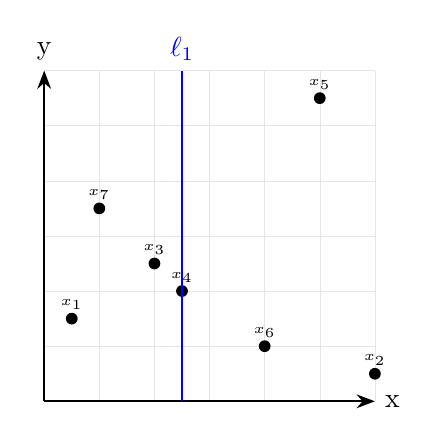
\begin{tikzpicture}[scale=0.35]
        % Grid
        \draw[very thin,gray!20] (0,0) grid[step=2] (12,12);
        \draw[->,thick] (0,0) -- (12,0) node[right] {x};
        \draw[->,thick] (0,0) -- (0,12) node[above] {y};
        
        % Points with labels
        \foreach \x/\y/\label in {
            1/3/1, 12/1/2, 4/5/3, 5/4/4, 10/11/5, 8/2/6, 2/7/7
        } {
            \node[circle,fill,inner sep=1.5pt] at (\x,\y) {};
            \node[font=\tiny] at (\x,\y+0.5) {$x_{\label}$};
        }
        
        % Splitting line
        \draw[blue,thick] (5,0) -- (5,12) node[above] {$\ell_1$};
    \end{tikzpicture}
    \caption*{Coordinate Split at Root Level}
    \end{figure}

    \item \textbf{Tree Structure}
    \begin{figure}[H]
    \centering
    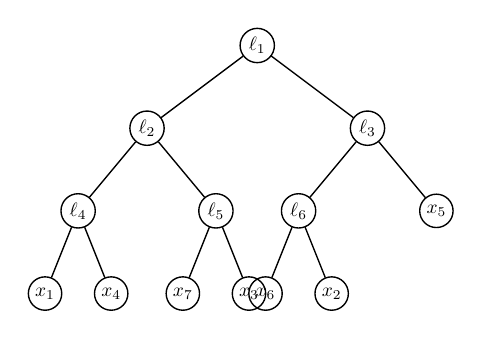
\begin{tikzpicture}[
        level distance=1.5cm,
        level 1/.style={sibling distance=4cm},
        level 2/.style={sibling distance=2.5cm},
        level 3/.style={sibling distance=1.2cm},
        scale=0.7,
        every node/.style={transform shape}
    ]
    \node [circle,draw,inner sep=2pt] {$\ell_1$}
        child {node [circle,draw,inner sep=2pt] {$\ell_2$}
            child {node [circle,draw,inner sep=2pt] {$\ell_4$}
                child {node [circle,draw,inner sep=2pt] {$x_1$}}
                child {node [circle,draw,inner sep=2pt] {$x_4$}}
            }
            child {node [circle,draw,inner sep=2pt] {$\ell_5$}
                child {node [circle,draw,inner sep=2pt] {$x_7$}}
                child {node [circle,draw,inner sep=2pt] {$x_3$}}
            }
        }
        child {node [circle,draw,inner sep=2pt] {$\ell_3$}
            child {node [circle,draw,inner sep=2pt] {$\ell_6$}
                child {node [circle,draw,inner sep=2pt] {$x_6$}}
                child {node [circle,draw,inner sep=2pt] {$x_2$}}
            }
            child {node [circle,draw,inner sep=2pt] {$x_5$}}
        };
    \end{tikzpicture}
    \caption*{KD-Tree Structure}
    \end{figure}
    \FloatBarrier

    \item \textbf{Final Properties}
    \begin{itemize}[noitemsep,leftmargin=*]
        \item Height: 3 (counting from 0)
        \item Leaves: 7 (all original points)
        \item Second leaf from left: $(4,5)$
    \end{itemize}
\end{enumerate}

\textbf{Exam Tips:}
\begin{enumerate}[noitemsep,leftmargin=*]
    \item Always start by sorting points on current dimension
    \item Mark median point clearly in your sorting
    \item Draw coordinate system with splitting lines
    \item Keep track of which dimension you're splitting on:
        \begin{itemize}[noitemsep,topsep=0pt]
            \item Level 0: x-coordinate
            \item Level 1: y-coordinate
            \item Level 2: x-coordinate
            \item And so on...
        \end{itemize}
    \item Verify tree properties at the end
\end{enumerate}

\textbf{Common Mistakes to Avoid:}
\begin{itemize}[noitemsep,leftmargin=*]
    \item Don't forget to alternate dimensions
    \item Don't skip sorting at each level
    \item Don't mix up left (<) and right (>) subtrees
    \item Don't forget to verify final tree properties
\end{itemize}

\FloatBarrier

\subsubsection{KD-Tree Complexity Analysis}
\textbf{Problem Type:} Complexity proof for KD-Tree construction

\textbf{What to Look For:}
\begin{itemize}[noitemsep,leftmargin=*]
    \item Proof of time complexity $O(n\log n)$
    \item Proof of space complexity $O(n)$
    \item Recursive analysis
\end{itemize}

\textbf{Solution Strategy:}
\begin{enumerate}[leftmargin=*,noitemsep]
    \item Prove space complexity first (easier)
    \item Analyze recursive structure
    \item Set up recurrence relation
    \item Apply Master Theorem
\end{enumerate}

\textbf{Space Complexity Proof:}
\begin{enumerate}[leftmargin=*,noitemsep]
    \item For $n = 2^k$ points:
        \begin{itemize}[noitemsep,topsep=0pt]
            \item Internal nodes (parents): $2^k - 1$
            \item Total nodes: $2^k + 2^{k-1} = n + n/2 = 3n/2 < 3n$
        \end{itemize}
    \item For general $n$ (not power of 2):
        \begin{itemize}[noitemsep,topsep=0pt]
            \item Find $t$ where $2^{t-1} < n < 2^t$
            \item Internal nodes $n_p$: $2^{t-2} < n_p < 2^{t-1}$
            \item Total nodes: $3 \cdot 2^{t-2} < n + n_p < 3 \cdot 2^{t-1}$
            \item Therefore: $n + n_p < 3n$
        \end{itemize}
    \item Each node uses $O(1)$ storage
    \item Total storage: $O(1) \cdot O(n) = O(n)$
\end{enumerate}

\textbf{Time Complexity Proof:}
\begin{enumerate}[leftmargin=*,noitemsep]
    \item At each recursion:
        \begin{itemize}[noitemsep,topsep=0pt]
            \item Split $n$ points into two subsets of $n/2$
            \item Finding median costs $O(n)$
        \end{itemize}
    \item Recurrence relation:
        \[ T(n) = \begin{cases}
            O(1) & \text{if } n = 1 \\
            2T(n/2) + O(n) & \text{if } n > 1
        \end{cases} \]
    \item Apply Master Theorem:
        \begin{itemize}[noitemsep,topsep=0pt]
            \item Similar to Merge-Sort analysis
            \item Results in $T(n) = O(n\log n)$
        \end{itemize}
\end{enumerate}

\textbf{Key Points for Exam:}
\begin{itemize}[noitemsep,leftmargin=*]
    \item Space complexity proof:
        \begin{itemize}[noitemsep,topsep=0pt]
            \item Count nodes for power of 2
            \item Extend to general case
            \item Multiply by constant storage
        \end{itemize}
    \item Time complexity proof:
        \begin{itemize}[noitemsep,topsep=0pt]
            \item Identify recursive pattern
            \item Write recurrence relation
            \item Apply Master Theorem
        \end{itemize}
    \item Remember median finding is $O(n)$
\end{itemize}

\textbf{Common Mistakes to Avoid:}
\begin{itemize}[noitemsep,leftmargin=*]
    \item Don't forget to account for non-power-of-2 cases
    \item Don't ignore constant factors in space analysis
    \item Remember to justify linear median finding
    \item Don't skip the Master Theorem application
\end{itemize}

\FloatBarrier

\subsubsection{Binary Search Trees (BST)}
\textbf{Definition:} A binary tree where for each node $x$:
\begin{itemize}[noitemsep,leftmargin=*]
    \item All keys in left subtree are < $x.key$
    \item All keys in right subtree are > $x.key$
    \item No duplicate keys allowed
\end{itemize}

\textbf{Basic Operations:}
\begin{enumerate}[noitemsep,leftmargin=*]
    \item \textbf{TREE-SEARCH$(x,k)$}: Find node with key $k$
        \begin{itemize}[noitemsep,topsep=0pt]
            \item Start at root, compare with $k$
            \item If equal: found
            \item If $k$ smaller: go left
            \item If $k$ larger: go right
            \item Time: $O(h)$ where $h$ is height
        \end{itemize}
    
    \item \textbf{TREE-MINIMUM$(x)$}: Find smallest key
        \begin{itemize}[noitemsep,topsep=0pt]
            \item Follow left pointers until NIL
            \item Time: $O(h)$
        \end{itemize}
    
    \item \textbf{TREE-MAXIMUM$(x)$}: Find largest key
        \begin{itemize}[noitemsep,topsep=0pt]
            \item Follow right pointers until NIL
            \item Time: $O(h)$
        \end{itemize}
    
    \item \textbf{TREE-SUCCESSOR$(x)$}: Find next larger key
        \begin{itemize}[noitemsep,topsep=0pt]
            \item If right subtree exists: TREE-MINIMUM(right)
            \item Else: Go up until first right turn
            \item Time: $O(h)$
        \end{itemize}
    
    \item \textbf{TREE-PREDECESSOR$(x)$}: Find next smaller key
        \begin{itemize}[noitemsep,topsep=0pt]
            \item If left subtree exists: TREE-MAXIMUM(left)
            \item Else: Go up until first left turn
            \item Time: $O(h)$
        \end{itemize}
\end{enumerate}

\textbf{Modifying Operations:}
\begin{enumerate}[noitemsep,leftmargin=*]
    \item \textbf{TREE-INSERT$(T,z)$}: Insert new node $z$
        \begin{itemize}[noitemsep,topsep=0pt]
            \item Follow BST property down to leaf
            \item Insert as left/right child
            \item Time: $O(h)$
        \end{itemize}
    
    \item \textbf{TREE-DELETE$(T,z)$}: Delete node $z$
        \begin{itemize}[noitemsep,topsep=0pt]
            \item Case 1: No children - remove directly
            \item Case 2: One child - replace with child
            \item Case 3: Two children:
                \begin{itemize}[noitemsep,topsep=0pt]
                    \item Find successor $y$ (min in right subtree)
                    \item Replace $z$ with $y$
                    \item Delete $y$ from original position
                \end{itemize}
            \item Time: $O(h)$
        \end{itemize}
\end{enumerate}

\textbf{Helper Operation:}
\begin{itemize}[noitemsep,leftmargin=*]
    \item \textbf{TRANSPLANT$(T,u,v)$}: Replace subtree
        \begin{itemize}[noitemsep,topsep=0pt]
            \item Replaces subtree rooted at $u$ with subtree rooted at $v$
            \item Updates parent pointers
            \item Used in DELETE operation
        \end{itemize}
\end{itemize}

\textbf{Properties:}
\begin{itemize}[noitemsep,leftmargin=*]
    \item Inorder traversal gives sorted sequence
    \item Height $h$ determines operation time:
        \begin{itemize}[noitemsep,topsep=0pt]
            \item Best case (balanced): $h = \lg n$
            \item Worst case (linear): $h = n$
        \end{itemize}
    \item No explicit balancing - shape depends on insertion order
\end{itemize}

\textbf{Tree Traversal:}
\begin{itemize}[noitemsep,leftmargin=*]
    \item \textbf{Inorder}: Left subtree → Root → Right subtree
        \begin{itemize}[noitemsep,topsep=0pt]
            \item Visits nodes in sorted order
            \item Used for ordered printing
        \end{itemize}
    \item \textbf{Preorder}: Root → Left subtree → Right subtree
        \begin{itemize}[noitemsep,topsep=0pt]
            \item Root processed before children
            \item Used for copying tree structure
        \end{itemize}
    \item \textbf{Postorder}: Left subtree → Right subtree → Root
        \begin{itemize}[noitemsep,topsep=0pt]
            \item Root processed after children
            \item Used for deletion
        \end{itemize}
\end{itemize}

\textbf{Implementation Details:}
\begin{itemize}[noitemsep,leftmargin=*]
    \item Node structure:
        \begin{itemize}[noitemsep,topsep=0pt]
            \item key: Value stored in node
            \item left, right: Pointers to children
            \item p: Pointer to parent (optional)
        \end{itemize}
    \item Sentinel NIL:
        \begin{itemize}[noitemsep,topsep=0pt]
            \item Used to mark leaf nodes
            \item Simplifies boundary conditions
        \end{itemize}
\end{itemize}

\textbf{Key Insights:}
\begin{itemize}[noitemsep,leftmargin=*]
    \item Successor never has left child
    \item Predecessor never has right child
    \item All operations maintain BST property
    \item Performance depends on tree height
    \item Balancing requires additional mechanisms (AVL, Red-Black)
\end{itemize}

\clearpage
\section{\texorpdfstring{\underline{Complexity Analysis}}{Complexity Analysis}}

\subsection{Sorting Complexity}
\textbf{Big-Oh Notation:} Describes the upper bound of an algorithm's running time. For example, $O(n \log n)$ is common in efficient sorting algorithms like Merge Sort.

\subsection{Quadratic Algorithms}
\textbf{Understanding $O(n^2)$:} Often seen in simple sorting algorithms like Bubble Sort, where each element is compared to every other element.

\subsection{Time Complexity}
\textbf{Complexity Classes:} Includes constant $O(1)$, logarithmic $O(\log n)$, linear $O(n)$, quadratic $O(n^2)$, and more. Helps in understanding the efficiency of algorithms.

\subsection{Dominant Terms}
\textbf{Identifying Dominant Terms:} In expressions like $5n^2 + 3n \log n$, the term $5n^2$ is dominant, leading to $O(n^2)$.

\subsection{Big-Oh Notation Properties}
\textbf{Rules:} Includes the rule of sums $O(f + g) = O(\max\{f, g\})$ and products $O(f \cdot g) = O(f) \cdot O(g)$.

\subsection{Computational Complexity}
\textbf{Nested Loops:} Analyzing loops within loops to determine total complexity, such as $O(n(\log n)^2)$ for certain nested structures.

\subsection{Master Theorem}
The Master Theorem provides a way to solve recurrence relations of the form:

\[ T(n) = aT\left(\frac{n}{b}\right) + f(n) \]

where $a \geq 1$, $b > 1$, and $f(n)$ is an asymptotically positive function. The theorem helps determine the asymptotic behavior of $T(n)$ by comparing $f(n)$ with $n^{\log_b a}$:

1. If $f(n) = O(n^{\log_b a - \epsilon})$ for some $\epsilon > 0$, then:
   \[ T(n) = \Theta(n^{\log_b a}) \]

2. If $f(n) = \Theta(n^{\log_b a})$, then:
   \[ T(n) = \Theta(n^{\log_b a} \log n) \]

3. If $f(n) = \Omega(n^{\log_b a + \epsilon})$ for some $\epsilon > 0$, and if $af(n/b) \leq cf(n)$ for some constant $c < 1$ and sufficiently large $n$, then:
   \[ T(n) = \Theta(f(n)) \]

The Master Theorem is widely used in analyzing the time complexity of divide-and-conquer algorithms, such as Merge Sort and Quick Sort.

\subsection{Heap Operations}
\textbf{Basic Heap Properties:}
\begin{itemize}
    \item A heap is a complete binary tree
    \item In a max-heap, for each node $i$: parent.key $\geq$ children.key
    \item In a min-heap, for each node $i$: parent.key $\leq$ children.key
\end{itemize}

\textbf{Array Representation:}
For a node at index $i$:
\begin{itemize}
    \item Parent: $\lfloor i/2 \rfloor$
    \item Left child: $2i$
    \item Right child: $2i + 1$
\end{itemize}

\begin{figure}[H]
    \centering
    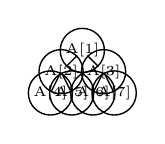
\begin{tikzpicture}[scale=0.45,
        level distance=0.6cm,
        level 1/.style={sibling distance=1.2cm},
        level 2/.style={sibling distance=0.6cm},
        every node/.style={circle,draw,inner sep=1pt,font=\tiny}]
        \node {A[1]}
            child {node {A[2]}
                child {node {A[4]}}
                child {node {A[5]}}
            }
            child {node {A[3]}
                child {node {A[6]}}
                child {node {A[7]}}
            };
    \end{tikzpicture}
    \caption*{\footnotesize Array indices in heap}
\end{figure}

\textbf{MAX-HEAPIFY Operation:}
\begin{enumerate}
    \item Compare root with children
    \item If child is larger, swap with largest child
    \item Recursively heapify affected subtree
\end{enumerate}

\begin{figure}[H]
    \centering
    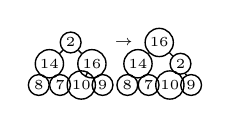
\begin{tikzpicture}[scale=0.45,
        level distance=0.6cm,
        level 1/.style={sibling distance=1.2cm},
        level 2/.style={sibling distance=0.6cm},
        every node/.style={circle,draw,inner sep=1pt,font=\tiny}]
        % Before MAX-HEAPIFY
        \node {2}
            child {node {14}
                child {node {8}}
                child {node {7}}
            }
            child {node {16}
                child {node {10}}
                child {node {9}}
            };
            
        % Arrow
        \node[draw=none] at (1.5,0) {$\rightarrow$};
        
        % After MAX-HEAPIFY
        \begin{scope}[xshift=2.5cm]
        \node {16}
            child {node {14}
                child {node {8}}
                child {node {7}}
            }
            child {node {2}
                child {node {10}}
                child {node {9}}
            };
        \end{scope}
    \end{tikzpicture}
    \caption*{\footnotesize MAX-HEAPIFY example}
\end{figure}

\textbf{BUILD-MAX-HEAP Operation:}
\begin{enumerate}
    \item Start from last non-leaf node ($\lfloor n/2 \rfloor$)
    \item Apply MAX-HEAPIFY to each node up to root
\end{enumerate}

\begin{figure}[H]
    \centering
    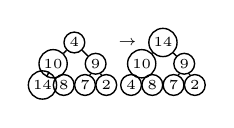
\begin{tikzpicture}[scale=0.45,
        level distance=0.6cm,
        level 1/.style={sibling distance=1.2cm},
        level 2/.style={sibling distance=0.6cm},
        every node/.style={circle,draw,inner sep=1pt,font=\tiny}]
        % Initial array as tree
        \node {4}
            child {node {10}
                child {node {14}}
                child {node {8}}
            }
            child {node {9}
                child {node {7}}
                child {node {2}}
            };
            
        % Arrow
        \node[draw=none] at (1.5,0) {$\rightarrow$};
        
        % After BUILD-MAX-HEAP
        \begin{scope}[xshift=2.5cm]
        \node {14}
            child {node {10}
                child {node {4}}
                child {node {8}}
            }
            child {node {9}
                child {node {7}}
                child {node {2}}
            };
        \end{scope}
    \end{tikzpicture}
    \caption*{\footnotesize BUILD-MAX-HEAP example}
\end{figure}

\textbf{HEAPSORT Operation:}
\begin{enumerate}
    \item BUILD-MAX-HEAP
    \item Repeatedly:
        \begin{itemize}[noitemsep,topsep=0pt]
            \item Swap root with last element
            \item Reduce heap size by 1
            \item MAX-HEAPIFY root
        \end{itemize}
\end{enumerate}
  
\clearpage
\section{\texorpdfstring{\underline{Graph Algorithms}}{Graph Algorithms}}
\subsection{Graph Representations}
\subsubsection{Graph Transpose}
\textbf{Problem Type:} Computing transpose $G^T$ of a directed graph $G=(V,E)$

\textbf{What to Look For:}
\begin{itemize}[noitemsep,leftmargin=*]
    \item Graph representation type (matrix/list)
    \item Direction of edges must be reversed
    \item Time complexity analysis required
\end{itemize}

\textbf{Key Definitions:}
\begin{itemize}[noitemsep,leftmargin=*]
    \item $G^T = (V,E^T)$ where $E^T = \{(v,u) \mid (u,v) \in E\}$
    \item $|V| = n$ (number of vertices)
    \item $|E|$ (number of edges)
\end{itemize}

\textbf{Solution for Adjacency Matrix:}
\begin{enumerate}[leftmargin=*,noitemsep]
    \item Given matrix $M_G$, create $M_G^T$ by swapping entries:
    \[ M = \begin{pmatrix}
        m_{11} & m_{12} & \cdots & m_{1n}\\
        m_{21} & m_{22} & \cdots & m_{2n}\\
        \vdots & \vdots & \ddots & \vdots\\
        m_{n1} & m_{n2} & \cdots & m_{nn}
    \end{pmatrix} \]
    
    \[ M^T = \begin{pmatrix}
        m_{11} & m_{21} & \cdots & m_{n1}\\
        m_{12} & m_{22} & \cdots & m_{n2}\\
        \vdots & \vdots & \ddots & \vdots\\
        m_{1n} & m_{2n} & \cdots & m_{nn}
    \end{pmatrix} \]

    \item Example:
    \[ M = \begin{pmatrix}1 & 2\\ 3 & 4\end{pmatrix}, 
       M^T = \begin{pmatrix}1 & 3\\ 2 & 4\end{pmatrix} \]
    
    \item Time Complexity: $\Theta(n^2)$
        \begin{itemize}[noitemsep]
            \item Must swap $n^2-n$ entries (excluding diagonal)
            \item Each swap is $O(1)$
        \end{itemize}
\end{enumerate}

\textbf{Solution for Adjacency List:}
\begin{enumerate}[leftmargin=*,noitemsep]
    \item Create empty adjacency lists for $G^T$: $O(n)$
    \item For each vertex $v$ in $G$:
        \begin{itemize}[noitemsep]
            \item For each edge $(v,w)$ in $v$'s adjacency list
            \item Add $v$ to $w$'s list in $G^T$
        \end{itemize}
    \item Time Complexity: $\Theta(|V| + |E|)$
        \begin{itemize}[noitemsep]
            \item Creating lists: $O(|V|)$
            \item Processing edges: $O(|E|)$
        \end{itemize}
\end{enumerate}

\textbf{Comparison:}
\begin{itemize}[noitemsep,leftmargin=*]
    \item Matrix: $\Theta(n^2)$ always
    \item List: $\Theta(|V| + |E|)$ which is better for sparse graphs
    \item List requires more complex implementation
\end{itemize}

\textbf{Common Mistakes to Avoid:}
\begin{itemize}[noitemsep,leftmargin=*]
    \item Don't forget self-loops (diagonal elements)
    \item Don't count diagonal elements in matrix swaps
    \item Remember to initialize all new lists in adjacency list solution
    \item Don't confuse $|V|$ and $|E|$ in complexity analysis
\end{itemize}

\FloatBarrier

\subsection{Shortest Paths}
\subsubsection{Dijkstra's Algorithm Limitations}
\textbf{Problem Type:} Counterexample for Dijkstra with negative weights

\textbf{What to Look For:}
\begin{itemize}[noitemsep,leftmargin=*]
    \item Directed graph with negative weights
    \item Minimal example showing algorithm failure
    \item Negative cycle demonstration
\end{itemize}

\textbf{Solution:}
\begin{enumerate}[leftmargin=*,noitemsep]
    \item Consider this directed graph:
    \begin{center}
    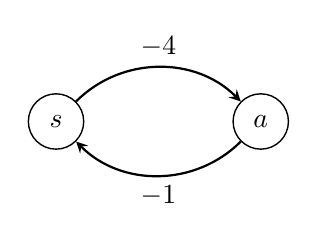
\begin{tikzpicture}[
        scale=1.3,
        vertex/.style={circle,draw,minimum size=20pt,inner sep=0pt}
    ]
        % Vertices
        \node[vertex] (s) at (0,0) {$s$};
        \node[vertex] (a) at (2,0) {$a$};
        
        % Curved edges
        \draw[thick,->,>=stealth] (s) to[bend left=45] node[above] {$-4$} (a);
        \draw[thick,->,>=stealth] (a) to[bend left=45] node[below] {$-1$} (s);
    \end{tikzpicture}
    \end{center}

    \item Why Dijkstra fails:
    \begin{itemize}[noitemsep]
        \item Initial distance to $a$: $-4$
        \item After one cycle: $-5$
        \item After two cycles: $-6$
        \item Continues to decrease indefinitely
    \end{itemize}
\end{enumerate}

\textbf{Key Properties:}
\begin{itemize}[noitemsep,leftmargin=*]
    \item Any negative cycle causes Dijkstra to fail
    \item Algorithm assumes:
        \begin{itemize}[noitemsep]
            \item Edge weights are non-negative
            \item Shortest paths exist (no negative cycles)
        \end{itemize}
    \item For negative weights, use Bellman-Ford instead
\end{itemize}

\textbf{Common Mistakes to Avoid:}
\begin{itemize}[noitemsep,leftmargin=*]
    \item Single negative edge isn't enough
    \item Example must have negative total cycle weight
\end{itemize}

\FloatBarrier


\clearpage
%\section{Exercises Part 1}

\subsection{Exercise 1.1: Sorting Complexity}
\textbf{Problem:} A sorting method with “Big-Oh” complexity $O(n \log n)$ spends exactly 1 millisecond to sort 1,000 data items. Given this, estimate how long it will take to sort 1,000,000 items.

\vspace{0.5em}
\textbf{Solution Steps:}
\begin{enumerate}[leftmargin=*,noitemsep]
    \item Understand the Problem: You need to find out how long it will take to sort 1,000,000 items using the given complexity.
    \item Identify Known Values:
    \begin{itemize}
        \item $T(1,000) = 1ms$
        \item Complexity is $O(n \log n)$
    \end{itemize}
    \item Calculate Constant $c$:
    \begin{itemize}
        \item Formula: $T(n) = c \cdot n \log n$
        \item Use $T(1,000) = 1ms$ to find $c$:
        \[ c = \frac{1ms}{1,000 \log 1,000} \]
    \end{itemize}
    \item Calculate $T(1,000,000)$:
    \begin{itemize}
        \item Use the formula $T(n) = c \cdot n \log n$
        \item Substitute $n = 1,000,000$:
        \[ T(1,000,000) = c \cdot 1,000,000 \cdot \log 1,000,000 \]
    \end{itemize}
    \item Simplify the Expression:
    \begin{itemize}
        \item Calculate $\log 1,000,000$
        \item Multiply and simplify to find the time in seconds.
    \end{itemize}
\end{enumerate}

\textbf{Exam Note:} Remember that $O(n \log n)$ complexity means the time increases logarithmically with the size of the data.

\textbf{Hint:} To solve similar exercises, focus on understanding the relationship between the given complexity and the time it takes to process a certain amount of data. Use the formula $T(n) = c \cdot f(n)$ to calculate the constant $c$ and then use it to find the time for a different amount of data.

\subsection{Exercise 1.2: Quadratic Algorithm}
\textbf{Problem:} A quadratic algorithm with processing time $T(n) = cn^2$ spends 1ms for 100 items. Calculate the time for 5,000 items.

\vspace{0.5em}
\textbf{Solution Steps:}
\begin{enumerate}[leftmargin=*,noitemsep]
    \item Understand the Problem: You need to calculate the time for 5,000 items given the complexity.
    \item Identify Known Values:
    \begin{itemize}
        \item $T(100) = 1ms$
        \item Complexity is $O(n^2)$
    \end{itemize}
    \item Calculate Constant $c$:
    \begin{itemize}
        \item Formula: $T(n) = c \cdot n^2$
        \item Use $T(100) = 1ms$ to find $c$:
        \[ c = \frac{1ms}{100^2} \]
    \end{itemize}
    \item Calculate $T(5,000)$:
    \begin{itemize}
        \item Use the formula $T(n) = c \cdot n^2$
        \item Substitute $n = 5,000$:
        \[ T(5,000) = c \cdot (5,000)^2 \]
    \end{itemize}
    \item Simplify the Expression:
    \begin{itemize}
        \item Calculate $(5,000)^2$
        \item Multiply and simplify to find the time in milliseconds.
    \end{itemize}
\end{enumerate}

\textbf{Exam Note:} Quadratic complexity $O(n^2)$ means time increases with the square of the data size.

\textbf{Hint:} To solve similar exercises, focus on understanding the relationship between the given complexity and the time it takes to process a certain amount of data. Use the formula $T(n) = c \cdot f(n)$ to calculate the constant $c$ and then use it to find the time for a different amount of data.

\FloatBarrier

\begin{table}[h]
    \centering
    \small
    \begin{tabularx}{\linewidth}{|X|X|X|}
        \hline
        Expression & Dominant term(s) & $O(\ldots)$ \\
        \hline
        5 + 0.001$n^3$ + 0.025$n$ & 0.001$n^3$ & $O(n^3)$ \\
        \hline
        500$n$ + 100$n^{1.5}$ + 50$n \log_{10} n$ & 100$n^{1.5}$ & $O(n^{1.5})$ \\
        \hline
        0.3$n$ + 5$n^{1.5}$ + 2.5 $\cdot$ $n^{1.75}$ & 2.5$n^{1.75}$ & $O(n^{1.75})$ \\
        \hline
        $n^2 \log_2 n$ + $n(n \log n)^2$ & $n^2 \log n$ & $O(n^2 \log n)$ \\
        \hline
        $n \log_3 n$ + $n \log_2 n$ & $n \log_3 n, n \log_2 n$ & $O(n \log n)$ \\
        \hline
        3 $\log_8 n$ + $\log_2 \log_2 \log_2 n$ & 3 $\log_8 n$ & $O(\log n)$ \\
        \hline
        100$n$ + 0.01$n^2$ & 0.01$n^2$ & $O(n^2)$ \\
        \hline
        0.01$n$ + 100$n^2$ & 100$n^2$ & $O(n^2)$ \\
        \hline
        2$n$ + $n^{0.5}$ + 0.5$n^{1.25}$ & 0.5$n^{1.25}$ & $O(n^{1.25})$ \\
        \hline
        0.01$n \log_2 n$ + $n(\log_2 n)^2$ & $n(\log_2 n)^2$ & $O(n(\log n)^2)$ \\
        \hline
        100$n \log_3 n$ + $n^3$ + 100$n$ & $n^3$ & $O(n^3)$ \\
        \hline
        0.003 $\log_4 n$ + $\log_2 \log_2 n$ & 0.003 $\log_4 n$ & $O(\log n)$ \\
        \hline
    \end{tabularx}
    \caption{Dominant terms and Big-Oh notation for various expressions.}
\end{table}

\begin{table}[h]
    \centering
    \small
    \begin{tabularx}{\linewidth}{|X|X|X|}
        \hline
        Statement & Is it TRUE or FALSE? & If it is FALSE then write the correct formula \\
        \hline
        Rule of sums: $O(f + g) = O(f) + O(g)$ & FALSE & $O(f + g) = \max\{O(f), O(g)\}$ \\
        \hline
        Rule of products: $O(f \cdot g) = O(f) \cdot O(g)$ & TRUE & \\
        \hline
        Transitivity: if $g = O(f)$ and $h = O(f)$ then $g = O(h)$ & FALSE & if $g = O(f)$ and $f = O(h)$ then $g = O(h)$ \\
        \hline
        $5n + 8n^2 + 100n^3 = O(n^4)$ & TRUE & \\
        \hline
        $5n + 8n^2 + 100n^3 = O(n^2 \log n)$ & FALSE & $5n + 8n^2 + 100n^3 = O(n^3)$ \\
        \hline
    \end{tabularx}
    \caption{Evaluation of Big-Oh notation statements.}
\end{table}

\begin{figure}[H]
    \centering
    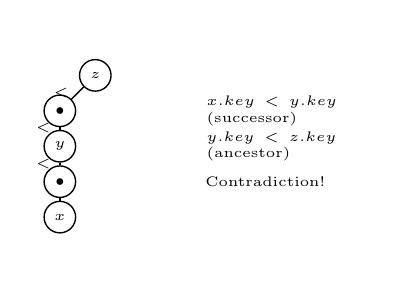
\begin{tikzpicture}[scale=0.45,
        level distance=1cm,
        level 1/.style={sibling distance=2cm},
        level 2/.style={sibling distance=1cm},
        every node/.style={circle,draw,inner sep=1pt,font=\tiny,minimum size=0.4cm}]
        
        % The tree showing contradiction
        \node (z) {$z$}
            child {
                node (leftz) {$\bullet$}
                child {
                    node (y) {$y$} 
                    child {
                        node (lefty) {$\bullet$}
                        child {
                            node (x) {$x$}
                        }
                        edge from parent node[left,draw=none,font=\tiny] {$<$}
                    }
                    edge from parent node[left,draw=none,font=\tiny] {$<$}
                }
                edge from parent node[left,draw=none,font=\tiny] {$<$}
            }
            child[missing];
            
        % Add explanatory text
        \node[draw=none,font=\tiny,text width=2cm,anchor=west] at (3,-1) 
            {$x.key < y.key$ (successor)};
        \node[draw=none,font=\tiny,text width=2cm,anchor=west] at (3,-2) 
            {$y.key < z.key$ (ancestor)};
        \node[draw=none,font=\tiny,text width=2cm,anchor=west] at (3,-3) 
            {Contradiction!};
    \end{tikzpicture}
    \caption*{\footnotesize Contradiction in BST property}
\end{figure}

\begin{figure}[H]
    \centering
    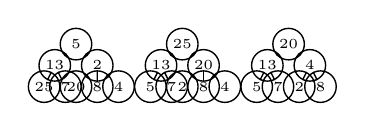
\begin{tikzpicture}[scale=0.45,
        level distance=0.6cm,
        level 1/.style={sibling distance=1.2cm},
        level 2/.style={sibling distance=0.6cm},
        level 3/.style={sibling distance=0.8cm},
        every node/.style={circle,draw,inner sep=1pt,font=\tiny,minimum size=0.4cm}]
        
        % Initial tree
        \node {5}
            child {node {13}
                child {node {25}}
                child {node {7}}
            }
            child {node {2}
                child {node {20}}
                child {node {8}}
                child {node {4}}
            };
            
        % After BUILD-MAX-HEAP
        \begin{scope}[xshift=3cm]
        \node {25}
            child {node {13}
                child {node {5}}
                child {node {7}}
            }
            child {node {20}
                child {node {2}}
                child {node {8}}
                child {node {4}}
            };
        \end{scope}
        
        % After first extraction
        \begin{scope}[xshift=6cm]
        \node {20}
            child {node {13}
                child {node {5}}
                child {node {7}}
            }
            child {node {4}
                child {node {2}}
                child {node {8}}
            };
        \end{scope}
    \end{tikzpicture}
    \caption*{\footnotesize HEAPSORT steps: Initial $\rightarrow$ BUILD-MAX-HEAP $\rightarrow$ First extraction}
\end{figure}

\sloppy

\subsection{Exercise 3.2: Tree Predecessor}
\textbf{Problem:} Write the TREE-PREDECESSOR procedure.

\textbf{Solution:} To obtain TREE-PREDECESSOR(x) procedure, we replace in TREE-SUCCESSOR(x) ``left'' instead of ``right'' and ``MAXIMUM'' instead of ``MINIMUM''.

\begin{algorithm}[H]
\begin{algorithmic}[1]
\Procedure{Tree-Predecessor}{$x$}
    \If{$x.right \neq \text{NIL}$}
        \State \Return Tree-Maximum($x.left$)
    \EndIf
    \State $y \gets x.p$
    \While{$y \neq \text{NIL}$ \textbf{and} $x = y.left$}
        \State $x \gets y$
        \State $y \gets y.p$
    \EndWhile
    \State \Return $y$
\EndProcedure
\end{algorithmic}
\end{algorithm}

\begin{figure}[H]
    \centering
    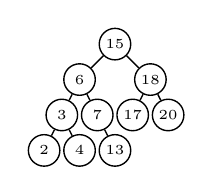
\begin{tikzpicture}[scale=0.45,
        level distance=1cm,
        level 1/.style={sibling distance=2cm},
        level 2/.style={sibling distance=1cm},
        every node/.style={circle,draw,inner sep=1pt,font=\tiny,minimum size=0.4cm}]
        
        % Example tree for predecessor
        \node {15}
            child {
                node {6}
                child {
                    node {3}
                    child {node {2}}
                    child {node {4}}
                }
                child {
                    node {7}
                    child[missing]
                    child {node {13}}
                }
            }
            child {
                node {18}
                child {node {17}}
                child {node {20}}
            };
    \end{tikzpicture}
    \caption*{\footnotesize Example: Predecessor of 15 is 13 (maximum in left subtree)}
\end{figure}

\textbf{Explanation:}
\begin{itemize}
    \item Case 1: If $x$ has a left subtree, the predecessor is the maximum element in that subtree
    \item Case 2: If no left subtree exists, we go up the tree until we find a node that is a right child
    \item The predecessor's key is the largest key in the tree smaller than $x.key$
\end{itemize}

\subsection{Exercise 3.4: Binary Search Tree Insertion}
\textbf{Problem:} Let $T$ be a Binary Search Tree. Prove that it always possible to insert a node $z$ as a leaf of the tree $T$ with $z.key = r$.

\textbf{Solution:} This is a straightforward property of Binary Search Trees. We prove this by induction on the height of the tree.

\begin{proof}
\begin{itemize}
\item \textbf{Base case} ($h = 0$):
    \begin{itemize}
        \item Tree consists only of root node $x$
        \item If $r \leq x.key$: place $z$ as left child of $x$
        \item If $r > x.key$: place $z$ as right child of $x$
    \end{itemize}

\item \textbf{Inductive step:}
    \begin{itemize}
        \item Assume the statement is true for trees of height $h-1$
        \item For a tree of height $h$ with root $x$:
        \begin{itemize}
            \item If $r \leq x.key$: insert in left subtree
            \item If $r > x.key$: insert in right subtree
        \end{itemize}
        \item By inductive hypothesis, we can insert in the chosen subtree (height $h-1$)
    \end{itemize}
\end{itemize}
\end{proof}

\begin{figure}[H]
    \centering
    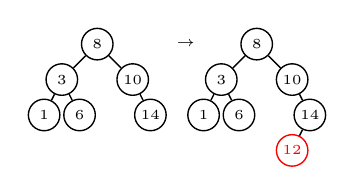
\begin{tikzpicture}[scale=0.45,
        level distance=1cm,
        level 1/.style={sibling distance=2cm},
        level 2/.style={sibling distance=1cm},
        every node/.style={circle,draw,inner sep=1pt,font=\tiny,minimum size=0.4cm}]
        
        % Before insertion
        \node {8}
            child {
                node {3}
                child {node {1}}
                child {node {6}}
            }
            child {
                node {10}
                child[missing]
                child {node {14}}
            };
            
        % Arrow
        \node[draw=none] at (2.5,0) {$\rightarrow$};
        
        % After insertion of 12
        \begin{scope}[xshift=4.5cm]
        \node {8}
            child {
                node {3}
                child {node {1}}
                child {node {6}}
            }
            child {
                node {10}
                child[missing]
                child {
                    node {14}
                    child {node[red] {12}}
                    child[missing]
                }
            };
        \end{scope}
    \end{tikzpicture}
    \caption*{\footnotesize Example: Inserting node with key=12 (shown in red)}
\end{figure}

\textbf{Key Points:}
\begin{itemize}
    \item The BST property ensures we can always find a valid leaf position
    \item At each step, we reduce the problem to a smaller subtree
    \item The process terminates when we reach a NULL child pointer
    \item Insertion maintains the BST property
\end{itemize}

\subsection{Exercise 3.5: Binary Search Tree Deletion}
\textbf{Problem:} Let $T$ be a Binary Search Tree given in the figure below. Give the output tree after the call of TREE-DELETE$(T, z)$ where $z$ is the node with key 41.

\begin{figure}[H]
    \centering
    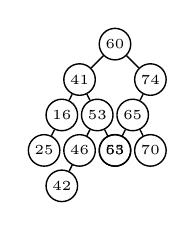
\begin{tikzpicture}[scale=0.45,
        level distance=1cm,
        level 1/.style={sibling distance=2cm},
        level 2/.style={sibling distance=1cm},
        every node/.style={circle,draw,inner sep=1pt,font=\tiny,minimum size=0.4cm}]
        
        % Initial tree
        \node {60}
            child {
                node {41}
                child {
                    node {16}
                    child {node {25}}
                    child[missing]
                }
                child {
                    node {53}
                    child {
                        node {46}
                        child {node {42}}
                        child[missing]
                    }
                    child {node {55}}
                }
            }
            child {
                node {74}
                child {
                    node {65}
                    child {node {63}}
                    child {node {70}}
                }
                child[missing]
            };
    \end{tikzpicture}
    \caption*{\footnotesize Initial Binary Search Tree with node 41 to be deleted}
\end{figure}

\textbf{Algorithm: TREE-DELETE$(T,z)$}
\begin{algorithm}[H]
\begin{algorithmic}[1]
\Procedure{Tree-Delete}{$T,z$}
    \If{$z.left = \text{NIL}$}
        \State \textsc{Transplant}$(T,z,z.right)$
    \ElsIf{$z.right = \text{NIL}$}
        \State \textsc{Transplant}$(T,z,z.left)$
    \Else
        \State $y \gets \text{Tree-Minimum}(z.right)$
        \If{$y.p \neq z$}
            \State \textsc{Transplant}$(T,y,y.right)$
            \State $y.right \gets z.right$
            \State $y.right.p \gets y$
        \EndIf
        \State \textsc{Transplant}$(T,z,y)$
        \State $y.left \gets z.left$
        \State $y.left.p \gets y$
    \EndIf
\EndProcedure
\end{algorithmic}
\end{algorithm}

\textbf{Solution:} Let's solve this step by step following the TREE-DELETE algorithm:

\begin{enumerate}
    \item \textbf{Analyze the node to be deleted (41):}
        \begin{itemize}
            \item Node 41 has two children: 16 (left) and 53 (right)
            \item Since it has two children, we fall into the third case (lines 7-15)
            \item We need to find its successor to replace it
        \end{itemize}
    
    \item \textbf{Find the successor of 41 (lines 7):}
        \begin{itemize}
            \item Call TREE-MINIMUM$(z.right)$ to find successor
            \item Right subtree starts at node 53
            \item Follow left pointers: 53 → 46 → 42
            \item Node 42 has no left child, so it's the successor
        \end{itemize}
    
    \item \textbf{Handle successor's position (lines 8-11):}
        \begin{itemize}
            \item Check if successor (42) is not a direct child of 41
            \item Since 42 is not direct child (it's grandchild), we:
                \begin{itemize}
                    \item Replace 42 with its right child (NIL in this case)
                    \item Make 42 point to 41's right child (53)
                    \item Make 53's parent point to 42
                \end{itemize}
        \end{itemize}

    \item \textbf{Complete the replacement (lines 12-14):}
        \begin{itemize}
            \item Replace 41 with 42 using TRANSPLANT
            \item Make 42 point to 41's left child (16)
            \item Make 16's parent point to 42
        \end{itemize}
\end{enumerate}

\begin{figure}[H]
    \centering
    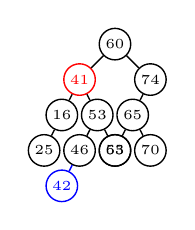
\begin{tikzpicture}[scale=0.45,
        level distance=1cm,
        level 1/.style={sibling distance=2cm},
        level 2/.style={sibling distance=1cm},
        every node/.style={circle,draw,inner sep=1pt,font=\tiny,minimum size=0.4cm}]
        
        % Intermediate step - finding successor
        \node {60}
            child {
                node[red] {41}
                child {
                    node {16}
                    child {node {25}}
                    child[missing]
                }
                child {
                    node {53}
                    child {
                        node {46}
                        child[blue] {node {42}}
                        child[missing]
                    }
                    child {node {55}}
                }
            }
            child {
                node {74}
                child {
                    node {65}
                    child {node {63}}
                    child {node {70}}
                }
                child[missing]
            };
    \end{tikzpicture}
    \caption*{\footnotesize Finding successor: Node to delete (41) in red, successor (42) in blue}
\end{figure}

\begin{figure}[H]
    \centering
    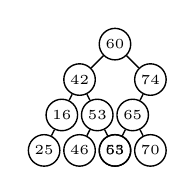
\begin{tikzpicture}[scale=0.45,
        level distance=1cm,
        level 1/.style={sibling distance=2cm},
        level 2/.style={sibling distance=1cm},
        every node/.style={circle,draw,inner sep=1pt,font=\tiny,minimum size=0.4cm}]
        
        % Final tree after deletion
        \node {60}
            child {
                node {42}
                child {
                    node {16}
                    child {node {25}}
                    child[missing]
                }
                child {
                    node {53}
                    child {
                        node {46}
                    }
                    child {node {55}}
                }
            }
            child {
                node {74}
                child {
                    node {65}
                    child {node {63}}
                    child {node {70}}
                }
                child[missing]
            };
    \end{tikzpicture}
    \caption*{\footnotesize Final Binary Search Tree after deleting node 41}
\end{figure}

\textbf{Key Points for Tree Deletion:}
\begin{itemize}
    \item There are three cases when deleting a node:
        \begin{enumerate}
            \item Node has no children (leaf node):
                \begin{itemize}
                    \item Simply remove it by setting parent's pointer to NIL
                    \item Example: Deleting a leaf like node 25
                \end{itemize}
            
            \item Node has one child:
                \begin{itemize}
                    \item Replace node with its only child
                    \item Update parent pointers
                    \item Example: If node 16 had only child 25
                \end{itemize}
            
            \item Node has two children:
                \begin{itemize}
                    \item Find successor (smallest value in right subtree)
                    \item Replace node with successor
                    \item Handle successor's original position
                    \item Example: Node 41 in our case
                \end{itemize}
        \end{enumerate}
    
    \item Finding the successor (TREE-MINIMUM):
        \begin{itemize}
            \item Start at node's right child
            \item Keep following left pointers until NIL
            \item Last node found is successor
            \item Important: Successor never has a left child
        \end{itemize}
    
    \item TRANSPLANT operation:
        \begin{itemize}
            \item Used to replace one subtree with another
            \item Updates parent pointers correctly
            \item Handles special case of root node
            \item Does not handle child pointers of moved nodes
        \end{itemize}
\end{itemize}

\textbf{Verification:} After deletion:
\begin{itemize}
    \item Node 42 maintains BST property:
        \begin{itemize}
            \item Left subtree (16, 25) contains values < 42
            \item Right subtree (53, 46, 55) contains values > 42
        \end{itemize}
    \item Tree structure remains valid:
        \begin{itemize}
            \item All parent-child pointers are correct
            \item No nodes were lost or duplicated
        \end{itemize}
    \item BST invariants are preserved:
        \begin{itemize}
            \item For every node: left subtree values < node key < right subtree values
            \item Tree remains connected
            \item No cycles are created
        \end{itemize}
\end{itemize}

\subsection{Exercise 4.1: Quicksort Partitioning Worst Case}
\textbf{Problem:} Prove that the worst case in Partitioning Algorithm (for Quicksort) has running time $\Theta(n^2)$, where $n$ is the cardinality of the set of elements in the partitioning.

\textbf{Solution:} We provide both an intuitive proof and a formal proof by induction.

\textbf{Part 1: Intuitive Proof}
\begin{enumerate}[leftmargin=*,noitemsep]
    \item \textbf{Worst Case Scenario:}
    \begin{itemize}[noitemsep]
        \item At each step, we get maximally unbalanced partitions:
        \item A $k-1$ element array and an empty array
        \item This happens when pivot is always smallest/largest element
    \end{itemize}

    \item \textbf{Recurrence Relation:}
    Let $T(n)$ be the running time of Quicksort with Partition:
    \begin{itemize}[noitemsep]
        \item Splitting time is linear: $\Theta(k)$ for array of size $k$
        \item Base case: $T(0)$ is constant, so $T(0) = \Theta(1)$
        \item For size $k$: $T(k) = T(k-1) + T(0) + \Theta(k)$
        \item Simplifies to: $T(k) = T(k-1) + \Theta(k)$
    \end{itemize}

    \item \textbf{Solving the Recurrence:}
    \begin{align*}
        T(n) &= T(n-1) + \Theta(n) \\
        &= T(n-2) + \Theta(n-1) + \Theta(n) \\
        &= T(n-3) + \Theta(n-2) + \Theta(n-1) + \Theta(n) \\
        &\vdots \\
        &= T(0) + \sum_{i=1}^n \Theta(i)
    \end{align*}

    \item \textbf{Final Step:}
    \begin{itemize}[noitemsep]
        \item Sum is arithmetic series: $\sum_{i=1}^n i$
        \item Using identity: $\sum_{i=1}^n i = \frac{n(n+1)}{2}$
        \item Therefore: $T(n) = \Theta(n^2)$
    \end{itemize}
\end{enumerate}

\textbf{Part 2: Formal Proof by Induction}
\begin{enumerate}[leftmargin=*,noitemsep]
    \item \textbf{Claim:} $T(n) = \Theta(n^2)$ for worst-case running time
    
    \item \textbf{Precise Statement:}
    \begin{itemize}[noitemsep]
        \item For all $0 < m < n$: $T(m) = \Theta(m^2)$
        \item This means $\exists c_1,d_1 > 0: c_1m^2 \leq T(m) \leq d_1m^2$
        \item Partition time $P(m) = \Theta(m)$, so $\exists c_2,d_2 > 0: c_2m \leq P(m) + T(0) \leq d_2m$
    \end{itemize}

    \item \textbf{Constants:}
    \begin{itemize}[noitemsep]
        \item Let $c = \min\{c_1,c_2\}$ and $d = \max\{d_1,d_2,1\}$
        \item Then for all $m \geq n-1$: $cm^2 \leq T(m) \leq dm^2$
        \item And for all $m \geq n$: $2cm \leq T(0) + P(m) \leq dm$
    \end{itemize}

    \item \textbf{Inductive Step:}
    \begin{align*}
        T(n) &= T(n-1) + T(0) + P(n) \\
        c(n-1)^2 + 2cn &\leq cn^2 - 2cn + 1 + 2cn = cn^2 + 1 \\
        d(n-1)^2 + dn &\leq dn^2 - dn + 1 \leq dn^2
    \end{align*}

    Therefore: $cn^2 < T(n) \leq dn^2$, proving $T(n) = \Theta(n^2)$
\end{enumerate}

\textbf{Key Insights:}
\begin{itemize}[noitemsep]
    \item The worst case occurs with extremely unbalanced partitions
    \item Each partition step costs linear time
    \item The cumulative effect leads to quadratic runtime
    \item Both intuitive and formal proofs confirm $\Theta(n^2)$ complexity
\end{itemize}

\subsection{Exercise 4.2: COUNTING-SORT Algorithm}
\textbf{Problem:} We apply COUNTING-SORT with the input vector $A = (5,6,5,3,3,7,4,4,4,5,3,8,8)$. Let $C$ and $B$ be the arrays mentioned in the pseudocode of COUNTING-SORT. Answer the following questions:

\begin{enumerate}[leftmargin=*,noitemsep]
    \item What is $C[7]$ after the for loop at lines 7-8 of the pseudocode?
    \item What is $B[13]$ after the first cycle at line 10?
    \item What is $C[8]$ after the first cycle?
\end{enumerate}

\textbf{Solution:} Let's solve this step by step following the COUNTING-SORT algorithm.

\textbf{1. Algorithm Overview:}
\begin{itemize}[noitemsep]
    \item Input array $A = (5,6,5,3,3,7,4,4,4,5,3,8,8)$ with $k=8$ (max value)
    \item Array $C[0..k]$ is used for counting and cumulative sums
    \item Array $B[1..n]$ will store the sorted output
\end{itemize}

\textbf{2. Step-by-Step Execution:}
\begin{enumerate}[leftmargin=*,noitemsep]
    \item \textbf{Initialize array $C$:}
    \begin{itemize}[noitemsep]
        \item Create $C[0..8]$ initialized to zeros
        \item $C = [0,0,0,0,0,0,0,0,0]$
    \end{itemize}

    \item \textbf{Count elements (lines 3-4):}
    \begin{itemize}[noitemsep]
        \item Count occurrences of each value in $A$
        \item After this step: $C = [0,0,0,3,3,3,1,1,2]$
        \item Meaning: three 3s, three 4s, three 5s, one 6, one 7, two 8s
    \end{itemize}

    \item \textbf{Compute cumulative sums (lines 5-6):}
    \begin{itemize}[noitemsep]
        \item Transform $C$ into cumulative counts
        \item $C = [0,0,0,3,6,9,10,11,13]$
        \item Therefore, $C[7] = 11$ (\textbf{Answer to Question 1})
    \end{itemize}

    \item \textbf{Build sorted array (lines 7-8):}
    \begin{itemize}[noitemsep]
        \item Process $A$ from right to left
        \item Place elements in $B$ based on $C$ values
        \item After first cycle (processing last element 8):
            \begin{itemize}[noitemsep]
                \item $B[13] = 8$ (\textbf{Answer to Question 2})
                \item $C[8]$ is decremented to 12 (\textbf{Answer to Question 3})
            \end{itemize}
        \item Final sorted array: $B = [3,3,3,4,4,4,5,5,5,6,7,8,8]$
    \end{itemize}
\end{enumerate}

\textbf{Key Insights:}
\begin{itemize}[noitemsep]
    \item The cumulative sum array $C$ helps maintain stability by tracking positions
    \item Processing from right to left ensures stability
    \item $C[i]$ represents the position after which the next element $i$ should be placed
    \item Each placement decrements the corresponding counter in $C$
\end{itemize}

\textbf{Final Answers:}
\begin{enumerate}[noitemsep]
    \item $C[7] = 11$
    \item $B[13] = 8$
    \item $C[8] = 12$
\end{enumerate}

\subsection{Exercise 5.1: BUILDKDTREE Algorithm}
\textbf{Problem:} We apply BUILDKDTREE$(P,0)$ to the following set $P$ of points in the plane:
\[ P = \{(1,3), (12,1), (4,5), (5,4), (10,11), (8,2), (2,7)\} \]

Answer the following questions:
\begin{enumerate}[leftmargin=*,noitemsep]
    \item Give the height of the tree
    \item How many leaves are there?
    \item The second leaf (starting from left) is the point with first coordinate...
\end{enumerate}

\textbf{Solution:} Let's solve this step by step following the BUILDKDTREE algorithm.

\textbf{1. Algorithm Review:}
\begin{itemize}[noitemsep]
    \item At even depths (0,2,...): split on x-coordinate (vertical line)
    \item At odd depths (1,3,...): split on y-coordinate (horizontal line)
    \item Each split creates a new level in the tree
    \item Points are recursively divided into left and right subsets
\end{itemize}

\textbf{2. Step-by-Step Construction:}
\begin{enumerate}[leftmargin=*,noitemsep]
    \item \textbf{Root Level (depth 0, x-split):}
    \begin{itemize}[noitemsep]
        \item Sort by x-coordinate: $(1,3), (2,7), (4,5), (5,4), (8,2), (10,11), (12,1)$
        \item Median point $(5,4)$ becomes root $\ell_1$
        \item Left subset: $\{(1,3), (2,7), (4,5)\}$
        \item Right subset: $\{(8,2), (10,11), (12,1)\}$
    \end{itemize}

    \item \textbf{Level 1 (depth 1, y-split):}
    \begin{itemize}[noitemsep]
        \item Left subset sorted by y: $(1,3), (4,5), (2,7)$
        \item Right subset sorted by y: $(12,1), (8,2), (10,11)$
        \item Medians $(2,7)$ and $(10,11)$ become nodes $\ell_2$ and $\ell_3$
    \end{itemize}

    \item \textbf{Level 2 (depth 2, x-split):}
    \begin{itemize}[noitemsep]
        \item Split remaining points into leaf nodes
        \item Left of $\ell_2$: $(1,3), (4,5)$ become leaves under $\ell_4$
        \item Left of $\ell_3$: $(8,2), (12,1)$ become leaves under $\ell_6$
    \end{itemize}
\end{enumerate}

\begin{figure}[H]
    \centering
    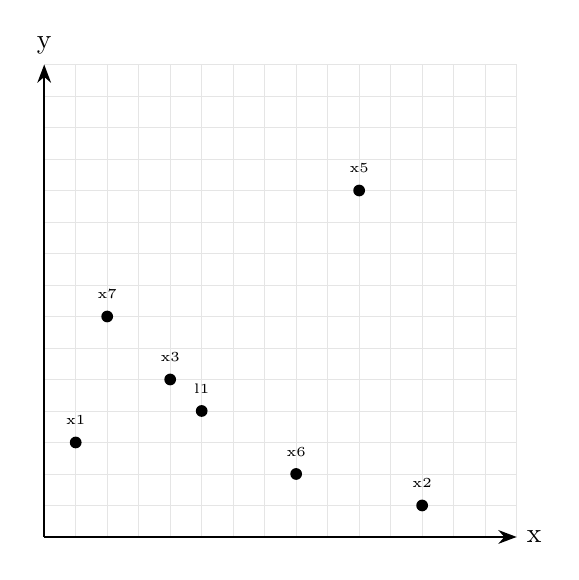
\begin{tikzpicture}[scale=0.4]
        % Grid
        \draw[very thin,gray!20] (0,0) grid (15,15);
        \draw[->,thick] (0,0) -- (15,0) node[right] {x};
        \draw[->,thick] (0,0) -- (0,15) node[above] {y};
        
        % Points with labels
        \node[circle,fill,inner sep=1.5pt] (x1) at (1,3) {};
        \node[font=\tiny] at (1,3.7) {x1};
        
        \node[circle,fill,inner sep=1.5pt] (x2) at (12,1) {};
        \node[font=\tiny] at (12,1.7) {x2};
        
        \node[circle,fill,inner sep=1.5pt] (x3) at (4,5) {};
        \node[font=\tiny] at (4,5.7) {x3};
        
        \node[circle,fill,inner sep=1.5pt] (x4) at (5,4) {};
        \node[font=\tiny] at (5,4.7) {l1};
        
        \node[circle,fill,inner sep=1.5pt] (x5) at (10,11) {};
        \node[font=\tiny] at (10,11.7) {x5};
        
        \node[circle,fill,inner sep=1.5pt] (x6) at (8,2) {};
        \node[font=\tiny] at (8,2.7) {x6};
        
        \node[circle,fill,inner sep=1.5pt] (x7) at (2,7) {};
        \node[font=\tiny] at (2,7.7) {x7};
    \end{tikzpicture}
    \caption*{Points in 2D plane}
\end{figure}

\begin{figure}[H]
    \centering
    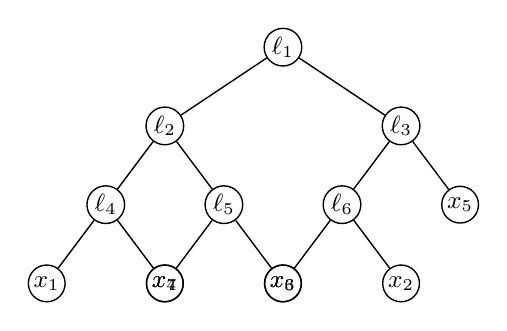
\begin{tikzpicture}[
        level distance=1cm,
        level 1/.style={sibling distance=3cm},
        level 2/.style={sibling distance=1.5cm},
        every node/.style={circle,draw,inner sep=1pt,font=\small}
    ]
        \node {$\ell_1$}
            child {node {$\ell_2$}
                child {node {$\ell_4$}
                    child {node {$x_1$}}
                    child {node {$x_4$}}
                }
                child {node {$\ell_5$}
                    child {node {$x_7$}}
                    child {node {$x_3$}}
                }
            }
            child {node {$\ell_3$}
                child {node {$\ell_6$}
                    child {node {$x_6$}}
                    child {node {$x_2$}}
                }
                child {node {$x_5$}}
            };
    \end{tikzpicture}
    \caption*{Final KD-Tree structure}
\end{figure}

\textbf{3. Answers:}
\begin{enumerate}[noitemsep]
    \item Height of the tree = 3 (counting levels from 0)
    \item Number of leaves = 7 (each original point becomes a leaf)
    \item Second leaf from left = $x_4 = (4,5)$
\end{enumerate}

\textbf{Key Insights:}
\begin{itemize}[noitemsep]
    \item The tree is built by alternating between x and y coordinates
    \item Each internal node represents a splitting line
    \item Vertical splits (even depths) compare x-coordinates
    \item Horizontal splits (odd depths) compare y-coordinates
    \item All original points end up as leaves
\end{itemize}

\subsection{Exercise 5.2: BUILDKDTREE Complexity}
\textbf{Problem:} (It is enough to give an intuitive idea) Prove that the BUILDKDTREE for a set of $n$ points has running time $O(n \log n)$ and uses $O(n)$ storage.

\textbf{Solution:} Let's break this down into two parts: storage complexity and runtime complexity.

\textbf{1. Storage Complexity $O(n)$:}
\begin{itemize}[noitemsep]
    \item Each splitting line divides points into two equal parts (up to unity)
    \item For $n = 2^k$ points, we need $2^k - 1$ lines (internal nodes)
    \item For splitting 2, the total nodes (parents + leaves) is:
        \[ 2^k + 2^{k-1} = n + n/2 = 3n/2 < 3n \]
    \item For $n$ not a power of 2, there exists $t$ where $2^{t-1} < n < 2^t$
    \item Number of internal nodes $n_p$ is bounded by:
        \[ 2^{t-2} < n_p < 2^{t-1} \]
    \item Total nodes (parents + leaves) satisfies:
        \[ 3 \cdot 2^{t-2} < n + n_p < 3 \cdot 2^{t-1} \]
    \item Therefore: $n + n_p < 3 \cdot 2^{t-1} < 3n$
    \item Each node uses $O(1)$ storage
    \item Total storage: $O(1) \cdot O(n) = O(n)$
\end{itemize}

\textbf{2. Runtime Complexity $O(n \log n)$:}
\begin{itemize}[noitemsep]
    \item BUILDKDTREE is recursive:
        \begin{itemize}[noitemsep]
            \item Each recursion splits $n$ points into two $n/2$ subsets
            \item Split cost is linear ($O(n)$): finding median in x or y coordinates
        \end{itemize}
    \item Building time $T(n)$ follows the recurrence:
        \[ T(n) = \begin{cases}
            O(1) & \text{if } n = 1 \\
            2T(n/2) + O(n) & \text{if } n > 1
        \end{cases} \]
    \item By Master Theorem (as in Merge-Sort):
        \begin{itemize}[noitemsep]
            \item $a = 2$ (subproblems)
            \item $b = 2$ (size reduction)
            \item $f(n) = O(n)$ (split cost)
            \item Case 1: $f(n) = O(n) = \Theta(n^{\log_2 2}) = \Theta(n)$
            \item Therefore: $T(n) = O(n \log n)$
        \end{itemize}
\end{itemize}

\textbf{Key Insights:}
\begin{itemize}[noitemsep]
    \item Storage is linear because each point becomes exactly one leaf node
    \item Runtime is $O(n \log n)$ due to:
        \begin{itemize}[noitemsep]
            \item Linear-time splitting at each level
            \item Logarithmic number of levels in the tree
        \end{itemize}
\end{itemize}

\begin{itemize}
    \item Example of a point $p_1$ \hfill
\end{itemize}

\begin{itemize}
    \item Example of a point $p_2$ \hfill
\end{itemize}

\begin{itemize}
    \item Example of a point $p_3$ \hfill
\end{itemize}

\begin{itemize}
    \item Example of a point $p_4$ \hfill
\end{itemize}

\begin{itemize}
    \item Example of a point $p_5$ \hfill
\end{itemize}

\subsection{Exercise 6.1: Graph Transpose}
\textbf{Problem:} The transpose of a directed graph $G = (V,E)$ is the graph $G^T = (V,E^T)$, where $E^T = \{(u,v) \mid (v,u) \in E\}$. Describe efficient algorithms for computing $G^T$ from $G$, for both the adjacency-list and adjacency-matrix representations of $G$. Analyze the running times of your algorithms.

\textbf{Solution:} Let's analyze both representations:

\textbf{1. Adjacency Matrix Representation:}
\begin{itemize}[noitemsep]
    \item Let $|V| = n$. If $M_G$ is the adjacency matrix of $G$, then $M_G^T$ is the adjacency matrix of $G^T$
    \item For a matrix $M$:
        \[ M = \begin{pmatrix}
            m_{11} & m_{12} & \cdots & m_{1n} \\
            m_{21} & m_{22} & \cdots & m_{2n} \\
            \vdots & \vdots & \ddots & \vdots \\
            m_{n1} & m_{n2} & \cdots & m_{nn}
        \end{pmatrix} \]
    \item The transpose matrix is:
        \[ M^T = \begin{pmatrix}
            m_{11} & m_{21} & \cdots & m_{n1} \\
            m_{12} & m_{22} & \cdots & m_{n2} \\
            \vdots & \vdots & \ddots & \vdots \\
            m_{1n} & m_{2n} & \cdots & m_{nn}
        \end{pmatrix} \]
    \item Example:
        \[ M = \begin{pmatrix}
            1 & 2 \\
            3 & 4
        \end{pmatrix}, \quad
        M^T = \begin{pmatrix}
            1 & 3 \\
            2 & 4
        \end{pmatrix} \]
    \item Algorithm:
        \begin{itemize}[noitemsep]
            \item Swap all pairs $(m_{ij}, m_{ji})$ outside main diagonal
            \item Number of swaps: $n^2 - n$ (excluding diagonal)
            \item Time complexity: $\Theta(n^2)$
        \end{itemize}
\end{itemize}

\textbf{2. Adjacency List Representation:}
\begin{itemize}[noitemsep]
    \item Algorithm:
        \begin{enumerate}[noitemsep]
            \item Create new "vertical list" with all vertices $V$ of $G^T$ (same as $G$)
                \begin{itemize}[noitemsep]
                    \item Cost: $\Theta(n)$
                \end{itemize}
            \item For each vertex $v$ in $G$'s adjacency list:
                \begin{itemize}[noitemsep]
                    \item For each vertex $w$ in $v$'s list:
                        \begin{itemize}[noitemsep]
                            \item Add $v$ to $w$'s list in $G^T$
                        \end{itemize}
                \end{itemize}
            \item Total cost: $\Theta(|V| + |E|)$
        \end{enumerate}
\end{itemize}

\textbf{Complexity Analysis:}
\begin{itemize}[noitemsep]
    \item Adjacency Matrix: $\Theta(n^2)$
        \begin{itemize}[noitemsep]
            \item Must process every cell in matrix
            \item Independent of number of edges
        \end{itemize}
    \item Adjacency List: $\Theta(|V| + |E|)$
        \begin{itemize}[noitemsep]
            \item Must process each vertex once
            \item Must process each edge once
            \item More efficient for sparse graphs
        \end{itemize}
\end{itemize}

\textbf{Key Insights:}
\begin{itemize}[noitemsep]
    \item For dense graphs ($|E| \approx |V|^2$), both representations have similar performance
    \item For sparse graphs ($|E| \ll |V|^2$), adjacency list is more efficient
    \item Space complexity matches time complexity for both representations
\end{itemize}

\subsection{Exercise 6.2: Dijkstra's Algorithm with Negative Weights}
\textbf{Problem:} Give a simple example of a directed graph with some negative-weight edges for which Dijkstra's algorithm produces incorrect answers.

\textbf{Solution:} Any directed graph containing a cycle with a negative total weight will cause Dijkstra's algorithm to produce incorrect answers. Here's a simple example:

\begin{figure}[H]
\centering
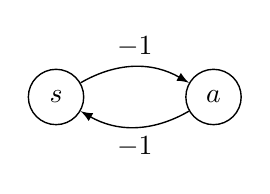
\begin{tikzpicture}[
    vertex/.style={circle,draw,minimum size=20pt,inner sep=0pt},
    >=latex
]
    % Vertices
    \node[vertex] (s) at (0,0) {$s$};
    \node[vertex] (a) at (2,0) {$a$};
    
    % Edges with weights
    \draw[->] (s) to[bend left=30] node[above] {$-1$} (a);
    \draw[->] (a) to[bend left=30] node[below] {$-1$} (s);
\end{tikzpicture}
\caption*{A graph with negative-weight cycle}
\end{figure}

\textbf{Why This Breaks Dijkstra's Algorithm:}
\begin{itemize}[noitemsep]
    \item Dijkstra's algorithm assumes that adding an edge to a path cannot decrease its total weight
    \item In this example:
        \begin{itemize}[noitemsep]
            \item Initial distance to $a$: $d[a] = -1$
            \item After one cycle: $d[a] = -3$
            \item After two cycles: $d[a] = -5$
            \item And so on...
        \end{itemize}
    \item The shortest path is undefined as we can keep traversing the cycle to get arbitrarily small path weights
\end{itemize}

\textbf{Key Insights:}
\begin{itemize}[noitemsep]
    \item Dijkstra's algorithm is guaranteed to work only with non-negative edge weights
    \item For graphs with negative weights, use the Bellman-Ford algorithm instead
    \item A negative cycle is detectable if after $|V|-1$ iterations, we can still relax an edge
    \item In practice, negative weights often indicate a modeling error in the problem
\end{itemize}

\subsection{Exercise 6.3: Dijkstra's Algorithm Iterations}
\textbf{Problem:} We apply DIJKSTRA (Lecture 13 and Lecture 14) to the following graph $(G,V)$ with starting node $a$. After INITIAL-SINGLE-SOURCE$(G,a)$ we have $a.d = 0$ and $v.d = \infty$ for each vertex $v \neq a$. What are the distances $c.d$, $f.d$, and $d.d$ after two iterations?

\begin{figure}[H]
\centering
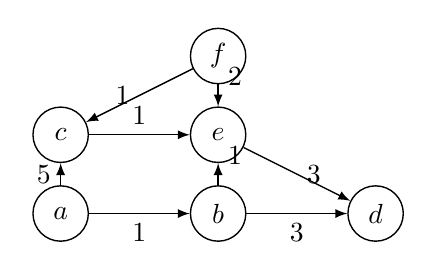
\begin{tikzpicture}[
    vertex/.style={circle,draw,minimum size=20pt,inner sep=0pt},
    >=latex
]
    % Vertices
    \node[vertex] (f) at (2,2) {$f$};
    \node[vertex] (c) at (0,1) {$c$};
    \node[vertex] (e) at (2,1) {$e$};
    \node[vertex] (a) at (0,0) {$a$};
    \node[vertex] (b) at (2,0) {$b$};
    \node[vertex] (d) at (4,0) {$d$};
    
    % Edges with weights
    \draw[->] (f) -- node[above right] {$2$} (e);
    \draw[->] (f) -- node[left] {$1$} (c);
    \draw[->] (c) -- node[above] {$1$} (e);
    \draw[->] (a) -- node[left] {$5$} (c);
    \draw[->] (a) -- node[below] {$1$} (b);
    \draw[->] (b) -- node[below] {$3$} (d);
    \draw[->] (b) -- node[above right] {$1$} (e);
    \draw[->] (e) -- node[right] {$3$} (d);
\end{tikzpicture}
\caption*{Graph for Dijkstra's Algorithm}
\end{figure}

\textbf{Solution:} Let's trace through the first two iterations:

\textbf{Initial State:}
\begin{itemize}[noitemsep]
    \item $a.d = 0$ (source)
    \item All other vertices: $v.d = \infty$
    \item $Q = \{a,b,c,d,e,f\}$
\end{itemize}

\textbf{First Iteration:}
\begin{itemize}[noitemsep]
    \item Extract-Min: vertex $a$ ($d = 0$)
    \item Relax edges from $a$:
        \begin{itemize}[noitemsep]
            \item $(a,b)$: $b.d = \min(\infty, 0 + 1) = 1$
            \item $(a,c)$: $c.d = \min(\infty, 0 + 5) = 5$
        \end{itemize}
    \item $Q = \{b,c,d,e,f\}$
\end{itemize}

\textbf{Second Iteration:}
\begin{itemize}[noitemsep]
    \item Extract-Min: vertex $b$ ($d = 1$)
    \item Relax edges from $b$:
        \begin{itemize}[noitemsep]
            \item $(b,d)$: $d.d = \min(\infty, 1 + 3) = 4$
            \item $(b,e)$: $e.d = \min(\infty, 1 + 1) = 2$
        \end{itemize}
    \item $Q = \{c,d,e,f\}$
\end{itemize}

\textbf{Final Answer:}
\begin{itemize}[noitemsep]
    \item $c.d = 5$ (from first iteration)
    \item $f.d = \infty$ (not yet reached)
    \item $d.d = 4$ (from second iteration)
\end{itemize}

\textbf{Key Insights:}
\begin{itemize}[noitemsep]
    \item Dijkstra's algorithm processes vertices in order of increasing distance
    \item After each iteration, distances are final for the processed vertex
    \item Unreachable vertices maintain distance $\infty$
    \item Each edge relaxation potentially updates the tentative distance to a vertex
\end{itemize}

\subsection{Exercise 7.1: Sorting by Polar Angle}
\textbf{Problem:} The polar angle of a point $p_i$ with respect to an origin $p_0$ is the angle from the semi-horizontal straight line $r$ and the vector $\overrightarrow{p_0p_i}$. The positive direction of the angle is counterclockwise. Angles are in the interval $[0, 2\pi)$. Write pseudocode to order $n$ points $q_1, \ldots, q_n$ by their polar angles in increasing order, with $O(n \log n)$ running time.

\textbf{Solution Strategy:}
\begin{enumerate}[noitemsep]
    \item Let $p_0 = [x_0, y_0]$ and $q_i = [x_i, y_i]$.
    \item Divide points $A = \{q_1, \ldots, q_n\}$ into:
        \begin{itemize}[noitemsep]
            \item $A_1$: Points with $y \geq y_0$
            \item $A_2$: Points with $y < y_0$
        \end{itemize}
    \item Polar angles in $A_1$ are in $[0, \pi]$, in $A_2$ are in $(\pi, 2\pi)$.
    \item Use ANGLEMEREGE-SORT to sort both $A_1$ and $A_2$.
\end{enumerate}

\textbf{Algorithm Details:}
\begin{itemize}[noitemsep]
    \item PARTITIONANGLE:
        \begin{itemize}[noitemsep]
            \item Purpose: Divides the array into two groups based on the y-coordinate relative to $y_0$.
            \item Process: Iterates through the array, swapping elements to ensure points in $A_1$ have polar angles in $[0, \pi]$ and points in $A_2$ in $(\pi, 2\pi)$.
            \item Complexity: $O(n)$, as each point is processed once.
        \end{itemize}
    \item ANGLEMERGE-SORT:
        \begin{itemize}[noitemsep]
            \item Purpose: Sorts points within each subset based on polar angles.
            \item Process: Uses a modified merge sort where the cross product is used to compare angles, ensuring correct order.
            \item Complexity: $O(n \log n)$, typical for merge sort algorithms.
        \end{itemize}
    \item ANGLE-SORT:
        \begin{itemize}[noitemsep]
            \item Purpose: Integrates the above methods to sort the entire set $A$.
            \item Process: Calls PARTITIONANGLE to separate the points, then applies ANGLEMEREGE-SORT to each subset.
            \item Complexity: $O(n \log n)$, combining the efficiencies of partitioning and sorting.
        \end{itemize}
\end{itemize}

\textbf{Pseudocode:}
\begin{verbatim}
procedure PARTITIONANGLE(A, y0):
    i = 0
    for j = 1 to n do
        if y.A[j] >= y0 then
            i = i + 1
            exchange A[i] with A[j]
    return i + 1

procedure ANGLEMEREGE-SORT(A, p, r):
    if p < r then
        q = (p + r) / 2
        ANGLEMEREGE-SORT(A, p, q)
        ANGLEMEREGE-SORT(A, q + 1, r)
        ANGLEMEREGE(A, p, q, r)

procedure ANGLE-SORT(A):
    if A != NIL then
        n = length.A
        q = PARTITIONANGLE(A, x0)
        ANGLEMEREGE-SORT(A, 1, q - 1)
        ANGLEMEREGE-SORT(A, q, n)
\end{verbatim}

\textbf{Complexity Analysis:}
\begin{itemize}[noitemsep]
    \item PARTITIONANGLE: $O(n)$
    \item ANGLEMEREGE-SORT: $O(n \log n)$
    \item Overall complexity: $O(n \log n)$
\end{itemize}

\textbf{Key Insights:}
\begin{itemize}[noitemsep]
    \item Sorting by polar angle requires careful handling of angle wrap-around.
    \item Efficient sorting is crucial for applications in computational geometry.
    \item Polar angles can be computed using $\text{atan2}(y_i - y_0, x_i - x_0)$.
\end{itemize}

\subsection{Exercise 7.3: ANY-SEGMENTS-INTERSECT}
\textbf{Problem:} Argue that \texttt{ANY-SEGMENTS-INTERSECT} works correctly even if three or more segments intersect at the same point.

\begin{center}
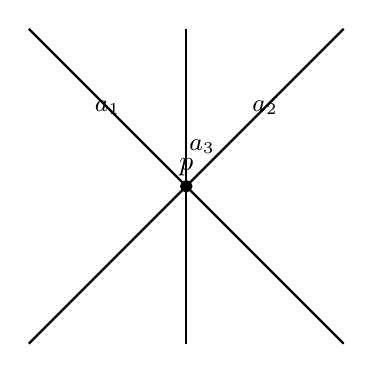
\begin{tikzpicture}
    \draw[thick] (0,0) -- (4,4);
    \draw[thick] (0,4) -- (4,0);
    \draw[thick] (2,0) -- (2,4);
    \node at (1,3) {\small $a_1$};
    \node at (3,3) {\small $a_2$};
    \node at (2.2,2.5) {\small $a_3$};
    \filldraw[black] (2,2) circle (2pt) node[anchor=south] {$p$};
\end{tikzpicture}
\end{center}

\textbf{Solution Strategy:}
\begin{enumerate}[noitemsep]
    \item Identify the conditions under which \texttt{ANY-SEGMENTS-INTERSECT} returns true.
    \item Analyze the behavior of the algorithm when three or more segments intersect.
    \item Prove correctness by considering event points and the sweep line.
\end{enumerate}

\textbf{Algorithm Details:}
\begin{itemize}[noitemsep]
    \item \textbf{Intersection Detection:}
        \begin{itemize}[noitemsep]
            \item Inserts a segment when it intersects with the above or below segment.
            \item Deletes a segment when its adjacent segments meet at a point.
        \end{itemize}
    \item \textbf{Event Point Analysis:}
        \begin{itemize}[noitemsep]
            \item Considers the first intersection point $p$ of $n$ segments.
            \item Analyzes the left and right points of segments at $p$.
        \end{itemize}
\end{itemize}

\textbf{Pseudocode Explanation:}
The pseudocode iterates through each event point, which represents either the start or end of a segment. When a left endpoint is encountered, the segment is added to the active set. If a right endpoint is reached, the segment is removed. The algorithm checks for intersections by evaluating if three or more segments meet at a point, returning true if so.

\textbf{Complexity Analysis:}
\begin{itemize}[noitemsep]
    \item Event processing: $O(n \log n)$
    \item Intersection checks: Efficient for multiple segments
\end{itemize}

\textbf{Key Insights:}
\begin{itemize}[noitemsep]
    \item The algorithm correctly identifies intersections involving multiple segments.
    \item The sweep line approach efficiently handles complex intersections.
\end{itemize}

\subsection{Exercise 7.4: ANY-SEGMENTS-INTERSECT with Vertical Segments}
\textbf{Problem:} Show that \texttt{ANY-SEGMENTS-INTERSECT} works correctly in the presence of vertical segments if we treat the bottom endpoint of a vertical segment as if it were a left endpoint and the top endpoint as if it were a right endpoint. How does your answer to Exercise 3 change if we allow vertical segments?

\begin{center}
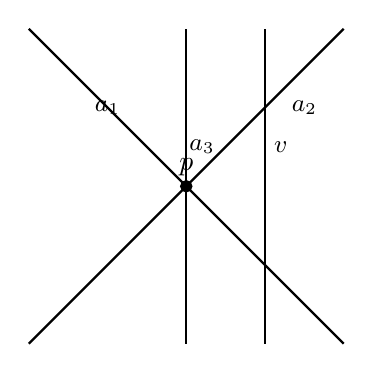
\begin{tikzpicture}
    \draw[thick] (0,0) -- (4,4);
    \draw[thick] (0,4) -- (4,0);
    \draw[thick] (2,0) -- (2,4);
    \draw[thick] (3,0) -- (3,4);
    \node at (1,3) {\small $a_1$};
    \node at (3.5,3) {\small $a_2$};
    \node at (2.2,2.5) {\small $a_3$};
    \node at (3.2,2.5) {\small $v$};
    \filldraw[black] (2,2) circle (2pt) node[anchor=south] {$p$};
\end{tikzpicture}
\end{center}

\textbf{Solution Strategy:}
\begin{enumerate}[noitemsep]
    \item Treat vertical segments with special rules for endpoints.
    \item Analyze how vertical segments affect the intersection detection.
    \item Prove correctness by considering vertical and non-vertical interactions.
\end{enumerate}

\textbf{Algorithm Details:}
\begin{itemize}[noitemsep]
    \item \textbf{Vertical Segment Handling:}
        \begin{itemize}[noitemsep]
            \item Treat the bottom endpoint as a left endpoint.
            \item Treat the top endpoint as a right endpoint.
        \end{itemize}
    \item \textbf{Intersection Detection:}
        \begin{itemize}[noitemsep]
            \item Check intersections with vertical segments using the sweep line.
            \item Ensure correct ordering of event points.
        \end{itemize}
\end{itemize}

\textbf{Pseudocode Explanation:}
The pseudocode processes each event point, treating vertical segment endpoints according to their roles. By treating the bottom as a left endpoint and the top as a right endpoint, the algorithm maintains the correct order and checks for intersections. This adjustment ensures that vertical segments are handled without altering the fundamental logic of the sweep line approach.

**Impact of Vertical Segments:** Allowing vertical segments in Exercise 7.3 would require treating their endpoints as described, ensuring that intersections involving vertical segments are detected correctly. The algorithm's logic remains intact, with the addition of handling vertical segment endpoints appropriately.

\textbf{Complexity Analysis:}
\begin{itemize}[noitemsep]
    \item Event processing: $O(n \log n)$
    \item Intersection checks: Efficient for vertical and non-vertical segments
\end{itemize}

\textbf{Key Insights:}
\begin{itemize}[noitemsep]
    \item The algorithm handles vertical segments by adjusting endpoint roles.
    \item The sweep line approach remains effective for complex intersections.
\end{itemize}

\end{multicols}

\section{Exercises Part 2}
\begin{multicols}{2}
\section{Exercises Part 2}
\subsection{Exercise 8.1: Drawing 5 Lines}
\textbf{Problem:} Prove that you cannot draw 5 lines on the Euclidean plane in such a way that each line cuts exactly 3 other lines.

\textbf{Solution:}
Using graph modeling:
\begin{itemize}
\item One line = one node
\item One intersection = one edge
\item Problem: Draw a graph with 5 nodes, each of degree 3
\item Sum of the degrees = 15
\item In any graph, sum of degrees must be even (each edge has 2 extremities)
\item Conclusion: Infeasible!
\end{itemize}

\textbf{Explanation:}
To solve similar problems, consider the following steps:
\begin{enumerate}
\item Model the problem using graph theory concepts.
\item Identify nodes and edges based on the problem statement.
\item Calculate the degree of each node and ensure the sum of degrees is even.
\item Use these calculations to determine feasibility.
\end{enumerate}

\subsection{Exercise 8.2: TSP Mathematical Formulation}
\textbf{Problem:} Give an exact formulation of the travelling salesperson problem.

\textbf{Solution:}
Input data:
\begin{itemize}
\item Distance matrix $D = (d_{ij})$ between cities $i$ and $j$
\item Objective: Find permutation $p$ of $n$ cities minimizing:
\[ \sum_{i=1}^{n-1} d_{p_ip_{i+1}} + d_{p_np_1} \]
\end{itemize}

\textbf{Explanation:}
For similar exercises:
\begin{enumerate}
\item Understand the problem constraints and objectives.
\item Define the input data clearly, such as distance matrices.
\item Formulate the objective function based on the problem requirements.
\item Use permutations or combinations to find optimal solutions.
\end{enumerate}

\subsection{Exercise 8.3: Cards Problem Optimization}
\textbf{Problem:} 50 cards numbered 1 to 50 must be separated into 2 stacks. First stack sum = 1170, second stack product = 36000.

\textbf{Solution:}
Encoding:
\begin{itemize}
\item Zero-one vector $s$ where $s_i = 0$ means card $i$ is in first stack
\item Objective function to minimize:
\[ f(s) = \left|\frac{1170 - \sum_{i=1}^{50} i \cdot (1-s_i)}{1170}\right| + \left|\frac{36000 - \prod_{i=1}^{50} i^{s_i}}{36000}\right| \]
\end{itemize}

\textbf{Explanation:}
For similar optimization problems:
\begin{enumerate}
\item Define the decision variables and constraints clearly.
\item Formulate the objective function to reflect the problem goals.
\item Use mathematical tools to solve for optimal solutions.
\item Validate results by checking against constraints.
\end{enumerate}

\subsection{Exercise 8.4: Timetable for Exams}
\textbf{Problem:} Timetable for Exams

\textbf{Solution:}
This problem can be formulated as a Vertex Colouring Problem: Each examination is a node, and two nodes are connected if at least one student exists who has to take both exams.

\textbf{Steps to Solve:}
\begin{enumerate}
\item \textbf{Identify Nodes:} Each exam is a node in the graph.
\item \textbf{Connect Nodes:} Draw an edge between nodes if a student is enrolled in both exams.
\item \textbf{Apply Colouring:} Use colouring to assign days to exams such that no two connected nodes share the same colour.
\item \textbf{Minimize Colours:} The goal is to use the minimum number of colours, representing the minimum number of days.
\end{enumerate}

\subsection{Exercise 8.5: Permutation Flow Shop Problem}
\textbf{Problem:} Number of Solutions for Permutation Flow Shop Problem

\textbf{Solution:}
For Permutation Flow Shop Problems, only the ordering of the n jobs on the first machine need to be selected, since the ordering of tasks on the other machines is then fixed. So there are n! permutations of n jobs.

\textbf{Steps to Solve:}
\begin{enumerate}
\item \textbf{Understand the Problem:} Recognize that the order of jobs on the first machine determines the sequence for all machines.
\item \textbf{Calculate Permutations:} Use factorial $n!$ to calculate the number of possible job sequences.
\item \textbf{Apply Constraints:} Consider any additional constraints that might affect the ordering.
\end{enumerate}

\subsection{Exercise 8.6: Asymptotic Runtime}
\textbf{Problem:} Asymptotic Runtime

\textbf{Solution:}
a) The asymptotic runtime of the given code is $O(n^2)$
b) The ascending ordering is: 1, log n, n, $n^2$, $n^3$, $(3/2)^n$, $2^n$.

\textbf{Steps to Solve:}
\begin{enumerate}
\item \textbf{Analyze Code:} Break down the loops to understand their contribution to runtime.
\item \textbf{Identify Dominant Terms:} Focus on the terms that grow fastest as $n$ increases.
\item \textbf{Order Functions:} Arrange functions by growth rate to understand their asymptotic behavior.
\end{enumerate}

\subsection{Exercise 8.7: Dijkstra's Algorithm}
\textbf{Problem:} Example on Dijkstra's Algorithm

\textbf{Solution:}
A, B, C, D, E
lambda = (0, 5, 2, 10, 12)
p = (-, C, A, B, D)

\textbf{Steps to Solve:}
\begin{enumerate}
\item \textbf{Initialize Distances:} Set the starting node's distance to zero and all others to infinity.
\item \textbf{Select Node:} Choose the node with the smallest tentative distance.
\item \textbf{Update Neighbors:} Calculate the tentative distances for neighboring nodes.
\item \textbf{Repeat:} Continue until all nodes are processed.
\item \textbf{Construct Path:} Use the predecessor array to reconstruct the shortest path.
\end{enumerate}

\subsection{Exercise 8.8: Prim's Algorithm}
\textbf{Problem:} Example on Prim's Algorithm

\textbf{Solution:}
A, B, C, D, E, F, G
lambda = (0, 7, 5, 5, 7, 6, 9)
p = (-, A, E, A, B, D, E)
$E_T$ = \{(A,D), (D,F), (A,B), (B,E), (E,C), (E,G)\}

\textbf{Steps to Solve:}
\begin{enumerate}
\item \textbf{Initialize:} Start with a single node and an empty edge set.
\item \textbf{Select Edge:} Choose the smallest edge connecting the tree to a new vertex.
\item \textbf{Add Edge:} Include this edge and vertex in the tree.
\item \textbf{Repeat:} Continue until all vertices are included in the tree.
\end{enumerate}

\end{multicols}

% Mock Exam Parts
\section{Mock Exam Part 1}
\begin{multicols}{2}
\newpage

% Mock Exam Part 1

\subsection{Exercise 1: Running Time}

\subsubsection*{Example 1}
1. (6P) Write the following Theta-classes in non-decreasing order from left to right (i.e., smallest on the left):

\(\Theta(n^2), \Theta(e^{\log_2 n}), \Theta(\sin n), \Theta(\ln^2 n), \Theta(\log_2 n), \Theta(n^3 + \ln(n^2)), \Theta(e^{n^2}), \Theta(e^{\ln(n^4)})\)

Solution: Understand growth rates: \(\sin n\) is slowest, followed by logarithmic, polynomial, and exponential. Use limits to compare and order.

2. (3P) We consider a recursive algorithm that involves an input with \(n\) objects and having running time \(T(n) = 4 \cdot T(n/2) + n^2\). Determine the running Theta class of the algorithm.

Solution: Identify recurrence: \(T(n) = a \cdot T(n/b) + f(n)\). Apply Master Theorem: Compare \(f(n)\) with \(n^{\log_b a}\) and determine the case.

3. (3P) We consider a recursive algorithm that involves an input with \(n\) objects and having running time \(T(n) = 4 \cdot T(n/2) + n\). Determine the running Theta class of the algorithm.

Solution: Apply Master Theorem: Use Case 1 for \(f(n) = O(n^{\log_b a - \epsilon})\).

4. (3P) We consider a recursive algorithm that involves an input with \(n\) objects and having running time \(T(n) = 4 \cdot T(n/2) + n^3\). Determine the running Theta class of the algorithm.

Solution: Apply Master Theorem: Use Case 3 for \(f(n) = \Omega(n^{\log_b a + \epsilon})\).

\subsubsection*{Solution:}
1. \(\Theta(\sin n), \Theta(\log_2 n), \Theta(\ln^2 n), \Theta(n^2), \Theta(e^{\log_2 n}), \Theta(n^3 + \ln(n^2)), \Theta(e^{\ln(n^4)}), \Theta(e^{n^2})\)

2. Case 2 Master theorem. \(\Theta(n^2 \ln n)\).

3. Case 1 Master theorem. \(\Theta(n^2)\).

4. Case 3 Master theorem. \(\Theta(n^3)\). (In all three cases, 1p corrected answer 2p correct justification)

\subsubsection*{Example 2}
1. (4P) Write in increasing order from left to right the following list of Theta classes. When two classes are equal, make it clear.

\(\Theta(n^{4/5}), \Theta(100n), \Theta(n \log_4 n), \Theta(n^{3/2}), \Theta(n^{\sqrt{n}}), \Theta(e^{\sqrt{2} \cdot n}), \Theta(e^n), \Theta(n!)\)

Solution: Understand growth rates: Familiarize yourself with common functions like polynomials, logarithms, exponentials, and factorials. Use limits to compare and order.

2. (2P) Give two functions \(f(n)\) and \(g(n)\) such that

\(\Theta(f(n) + g(n)) \neq \Theta(f(n))\) and \(\Theta(f(n) + g(n)) \neq \Theta(g(n))\)

Solution: Choose functions with different growth rates.

\subsubsection*{Solution:}
\(\Theta(n^{4/5}), \Theta(100n), \Theta(n \log_4 n), \Theta(n^{\sqrt{n}}), \Theta(n^{3/2}) = \Theta(n^{\sqrt{n}}), \Theta(e^n), \Theta(e^{\sqrt{2} \cdot n}), \Theta(n!)\)

\(f(n) = n\) and \(g(n) = -n + 1\)

\subsection*{Exercise 2: Pseudocode Examples}

\subsubsection*{Example 1: Pseudocode}

1. (6P) Write a pseudocode, which takes the input $A = \{a_1,a_2,\ldots,a_n\}$ and gives you as output $B = \{a_n,\ldots,a_2,a_1\}$ (i.e. same entries as in $A$ but, in the reversed order).

Solution approach:
- Use array indexing to swap elements
- Only need to iterate through half the array (why? because each swap handles two positions)
- Track running time: each operation is constant time, done n/2 times

\begin{verbatim}
REVERSEARRAY(A)
for i = 1 to ⌊n/2⌋
    exchange A[i] with A[n-i+1]
return A
\end{verbatim}

Running time: $\Theta(n)$ because we perform n/2 constant-time operations.

2. (9P) Let $S$ be a set with $n$ integers, randomly ordered and not necessarily distinct. Let $m$ be an integer. Write a pseudocode, which tests whether there are two elements $a,b \in S$ with $a + b = m$ (a and b may be the same number).

Solution approach:
- Naive solution: Check all pairs with nested loops = $O(n^2)$
- Better solution: Sort first, then use two pointers = $O(n \log n)$
- Best solution: Single pass with smart pointer movement = $O(n)$

Naive solution (for understanding):
\begin{verbatim}
SUMTEST(S,m)
for i = 1 to n-1
    for j = i+1 to n
        if S[i] + S[j] = m return true
return false
\end{verbatim}

Optimized solution:
\begin{verbatim}
SUMTESTBEST(S,m)
i = 1 to j = n
if S[i] + S[j] = m return true
if S[i] + S[j] < m, i=i+1
else j = j+1 (# that is if S[i] + S[j] > m)
stop when returns true or i > j
\end{verbatim}

Key insights for optimization:
- Avoid checking all pairs
- Use array properties to skip unnecessary checks
- Think about how to move pointers based on sum comparison with target
- Running time improves from $O(n^2)$ to $O(n)$

\subsection*{Exercise 3: Sweep Line Algorithm}

\subsubsection*{Example 1: ANYSEGMENTINTERSECT}

Given the algorithm ANYSEGMENTINTERSECT and line segments on an (x,y)-plane, determine the sweep lines and partial orders.

Solution approach:
1. Understand the algorithm:
   - Sorts endpoints from left to right
   - Maintains partial order of segments crossing sweep line
   - Checks for intersections at each event point

2. Steps to solve:
   a) First, identify all endpoints (left and right) of segments
   b) Sort them from left to right
   c) For each vertical sweep line at these points:
      - Draw the vertical line
      - List segments crossing this line from bottom to top
      - Check for intersections between adjacent segments

3. Key points to remember:
   - Left endpoint: INSERT segment into order
   - Right endpoint: DELETE segment from order
   - Check ABOVE and BELOW neighbors for intersections
   - Stop when intersection found

4. Example solution format:
   Sweep line at x = -2:
   Segments (bottom to top): a, f
   
   Sweep line at x = -1:
   Segments: a, e, f, b
   
   Sweep line at x = 0:
   Segments: c, e, f, b

Running time analysis:
- Sorting endpoints: $O(n \log n)$
- Each endpoint processed once: $O(n)$
- Total: $O(n \log n)$

Common mistakes to avoid:
- Don't forget to order segments from bottom to top
- Check both ABOVE and BELOW at insertion
- List ALL segments crossing each sweep line

\subsection*{Exercise 4: Points on the Plane}

\subsubsection*{Example 1: Points on the Plane}

1. (9P) Check for collinear points in 2D plane:

Solution steps:
a) For each point $p_0$ as center:
   - Calculate angles between $\overline{p_0p_1}$ and all other segments $\overline{p_0p_j}$
   - Use DIRECTION($p_0$, $p_i$, $p_j$) = cross product $(p_1 - p_0) \times (p_j - p_0)$
   - Calculate angle: $\alpha_j = \sin^{-1}(\frac{\text{cross product}}{||p_1-p_0|| \cdot ||p_j-p_0||})$

b) For each center point:
   - Sort angles using merge sort: $O(n \log n)$
   - Use SUMTESTBEST to find angles with 0 or $\pi$ difference: $O(n)$
   - Three points collinear if difference is 0 or $\pi$

Total running time: $O(n^2 \log n)$ because:
- Repeat for each point: $O(n)$
- For each center: $O(n \log n)$ for sorting + $O(n)$ for checking
- Final complexity: $n \cdot O(n \log n) = O(n^2 \log n)$

2. (6P) BUILDKDTREE construction:

Steps to construct KD-Tree:
a) Start with depth 0 (vertical split)
   - Find median x-coordinate
   - Split points into left/right sets

b) At depth 1 (horizontal split):
   - Find median y-coordinate in each subset
   - Split into top/bottom sets

c) Continue alternating between:
   - Even depth: vertical splits (x-coordinate)
   - Odd depth: horizontal splits (y-coordinate)

Example tree structure:
\begin{verbatim}
At root (depth 0): vertical split
- Left child: points left of median
- Right child: points right of median
  At depth 1: horizontal splits
  - Top/bottom division for each subset
\end{verbatim}

Key insights:
- Alternate between x and y coordinates based on depth
- Always split through median point
- Each split divides remaining points roughly in half
- Tree will be balanced if splits are perfect medians

\subsection*{Exercise 5: Fibonacci Sequence Analysis}

Input: Positive integer $n > 2$

Algorithm analysis:
\begin{verbatim}
INPUT: a positive integer n > 2
Create A an empty array with n entries
Set A[1] = A[2] = 1
for (i = 3; i ≤ n) do
    A[i] = A[i-1] + A[i-2]
return A[n]
\end{verbatim}

Solution steps:
- Algorithm builds Fibonacci sequence: 1, 1, 2, 3, 5, 8, 13, ...
- Each number is sum of previous two
- For n = 5, output is (1, 1, 2, 3, 5)
- Running time: $\Theta(n)$ as we do n-3 iterations with constant operations

\subsection*{Exercise 6: Binary Search Implementation}

Write a recursive algorithm (divide-and-conquer) to check if k is in sorted array A.

Solution approach:
1. Decomposition:
   - Find middle element
   - Compare k with middle
   - Determine which half to search

2. Implementation:
\begin{verbatim}
BINARYSEARCH(A, k, left, right)
    if left > right return -1
    mid = ⌊(left + right)/2⌋
    if A[mid] = k return mid
    if A[mid] > k
        return BINARYSEARCH(A, k, left, mid-1)
    return BINARYSEARCH(A, k, mid+1, right)
\end{verbatim}

Running time: $\Theta(\log n)$ because:
- Each step divides problem size by 2
- Constant work at each level
- Tree height is $\log n$

\subsection*{Exercise 7: Minimum Distance Algorithm}

Algorithm analysis for finding minimum distance between points:
\begin{verbatim}
INPUT: n ≥ 2 points (x₁,y₁), (x₂,y₂) ..., (xₙ,yₙ)
a = √((x₁-x₂)² + (y₁-y₂)²)
for (i = 1; i < n) do
    for (j = i+1; j ≤ n) do
        r = √((xᵢ-xⱼ)² + (yᵢ-yⱼ)²)
        if (r < a) then
            a = r
return a
\end{verbatim}

Solution analysis:
- Computes distance between all pairs of points
- Updates minimum distance when smaller distance found
- Running time: $\Theta(n^2)$ due to nested loops
- Space complexity: $\Theta(1)$ as only storing minimum distance

\subsection*{Exercise 8: Dijkstra's Algorithm}

\subsubsection*{Example 1: Dijkstra's Algorithm}

Consider weighted oriented graph with adjacency matrix:
\[
\begin{pmatrix}
    & s & x & y & z & w \\
s & 0 & 2 & 3 & 0 & 0 \\
x & 0 & 0 & 0 & 1 & 5 \\
y & 0 & 0 & 0 & 4 & 0 \\
z & 0 & 0 & 0 & 0 & 3 \\
w & 0 & 0 & 0 & 0 & 2
\end{pmatrix}
\]

Steps for Dijkstra's Algorithm:
1. Initialize:
   - Set source distances (s: 0, others: ∞)
   - Q = V (all vertices in queue)
   - S = ∅ (empty set of processed vertices)

2. Main loop:
   - Extract min from Q
   - Add to S
   - Update neighbors' distances
   - Track predecessors

3. Key points to remember:
   - Black vertices: in S (processed)
   - White vertices: in Q (unprocessed)
   - Grey vertex: current EXTRACT-MIN(Q)
   - Shaded edges: show predecessor values

\subsection*{Exercise 9: KD-Tree Construction}

\subsubsection*{Example 1: KD-Tree Construction}

Given points in xy-plane: $(-5,5), (-4,3), (-3,-5), (-2,-1), (-1,0), (0,-3), (1,2), (2,-4), (3,6)$

Steps to construct KD-Tree:
1. Depth 0 (vertical split):
   - Sort by x-coordinate
   - Find median x value
   - Split points into left/right sets

2. For each subset at depth 1:
   - Sort by y-coordinate
   - Split into top/bottom

3. Implementation tips:
   - Even depth: vertical split (x-coord)
   - Odd depth: horizontal split (y-coord)
   - Always include median in split
   - Balance tree by choosing true median

4. Visualization:
   - Draw vertical/horizontal lines at splits
   - Show points in resulting regions
   - Connect nodes based on splits
   - Label depth and split direction

\subsection*{Example 7: Array Operations}

1. Check for duplicates in array:
\begin{verbatim}
DUPLICATES(A)
    found = false
    for i from 1 to n-1
        for j=i+1 to n
            if a[i]=a[j] found=true
    return found
\end{verbatim}
Running time: $\Theta(n^2)$ because we check $\frac{n(n-1)}{2}$ pairs

2. Recursive sum of array segment:
\begin{verbatim}
Sum(a,l,r)
    if l=r
        return a[l]
    else
        centre=⌊(l+r)/2⌋
        sum1 = Sum(a,l,c)
        sum2 = Sum(a,c+1,r)
        return sum1+sum2
\end{verbatim}
Running time analysis:
- T(1) = c (constant time)
- T(n) = 2T(n/2) + O(1)
- By Master Theorem (Case 1): T(n) = Θ(n)

\subsection*{Example 8: Binary Search Tree Operations}

Tree-Delete operation steps:
1. Find node to delete
2. If leaf: simply remove
3. If one child: replace with child
4. If two children:
   - Find successor (minimum in right subtree)
   - Replace node with successor
   - Delete successor from original position

Key insights:
- Maintain BST properties after deletion
- Handle all cases (0, 1, 2 children)
- Track parent pointers for clean deletion

\subsection*{Example 9: Segment Intersections}

For segments between two parallel lines (y=0 and y=1):

Algorithm approach:
1. Sort points by x-coordinate
2. Count inversions to find intersections
3. Use divide-and-conquer:
   - Split into halves
   - Count inversions in each half
   - Merge and count cross-inversions

Running time analysis:
- T(n) = 2T(n/2) + O(n)
- By Master Theorem: T(n) = O(n log n)

Key optimization:
- Sort once at beginning
- Use merge-sort principle for counting
- Avoid checking all pairs (would be O(n²))

\end{multicols}

\section{Mock Exam Part 2}
\begin{multicols}{2}
\subsection{Question 1: Knapsack Problem}
\textbf{Question:} For a Knapsack Problem instance with \( n \) items and weight limit \( W \), a neighborhood is defined as follows: Remove the item with the worst value-to-weight ratio from the knapsack and then randomly insert an item that fits into (i.e., such that the weight limit is not exceeded). What is the best upper bound for the size of this neighborhood?

\textbf{Solution:}
The best upper bound for the size of this neighborhood is \( O(n^2) \).

\textbf{Explanation:}
To understand why the upper bound is \( O(n^2) \), consider the following:

1. **Value-to-Weight Ratio**: The value-to-weight ratio is a measure of how much value an item provides per unit of weight. Removing the item with the worst ratio means optimizing the knapsack's efficiency.

2. **Neighborhood Size**: After removing one item, you can potentially add any of the remaining \( n-1 \) items, provided they fit within the weight limit. This gives a linear number of choices.

3. **Combinatorial Nature**: Since you can remove any item and then add any other item, this results in a quadratic number of combinations, hence the \( O(n^2) \) complexity.

4. **Generalization**: Even if the question is framed differently, focus on the process of removing and adding items and the combinatorial possibilities to determine the neighborhood size.

\subsection{Question 2: Partially Mapped Crossover (PMX)}
\textbf{Question:} We apply Partially Mapped Crossover to the following permutations with swapping positions 4 to 7 (in blue):

P1: 9 3 1 \textcolor{blue}{7 4 6 2} 5 8\\
P2: 6 4 2 \textcolor{blue}{9 8 7 5} 3 1

\textbf{Solution:}
O1: 6 3 1 9 8 7 5 2 4\\
O2: 9 8 5 7 4 6 2 3 1

\textbf{Explanation:}
To solve PMX problems, follow these steps:

1. \textbf{Identify the Crossover Section:}
   - Positions 4-7 are swapped (blue section)
   - For O1: Take positions 4-7 from P2 (9875)
   - For O2: Take positions 4-7 from P1 (7462)

2. \textbf{Create Mapping:}
   - 7 \( \leftrightarrow \) 9
   - 4 \( \leftrightarrow \) 8
   - 6 \( \leftrightarrow \) 7
   - 2 \( \leftrightarrow \) 5

3. \textbf{Fill Remaining Positions:}
   - For positions outside the crossover section:
     * If the number from the original parent doesn't create a duplicate, keep it
     * If it would create a duplicate, use the mapping to find a replacement

\subsection{Question 3: Algorithmic Concepts (True/False)}
\textbf{Question:} For each statement, determine if it's True, False, or Not sure.

\begin{enumerate}[label=\alph*)]
\item TSP instances with up to 50 cities are most easily solved by an Exhaustive Search.\\
\textbf{Answer:} False\\
\textbf{Explanation:} While exhaustive search will find the optimal solution, it's not the most efficient approach even for 50 cities. The time complexity would be O(n!), making it impractical. Dynamic programming or branch-and-bound algorithms would be more efficient for this size.

\item If a problem is NP-hard, then it is in NP.\\
\textbf{Answer:} False\\
\textbf{Explanation:} This is a common misconception. NP-hard problems are at least as hard as the hardest problems in NP, but they don't necessarily have to be in NP themselves. For example, the halting problem is NP-hard but not in NP.

\item The Steiner Tree Problem is similar to the Minimum Spanning Tree Problem and can hence be solved in polynomial time.\\
\textbf{Answer:} False\\
\textbf{Explanation:} While both problems involve connecting nodes in a graph, the Steiner Tree Problem is NP-hard, unlike the Minimum Spanning Tree Problem which can be solved in polynomial time (e.g., using Kruskal's or Prim's algorithm).

\item In the Capacitated Vehicle Routing Problem (CVRP), the location of the depot is usually fixed.\\
\textbf{Answer:} True\\
\textbf{Explanation:} In the standard CVRP, the depot location is indeed fixed. The problem focuses on finding optimal routes for vehicles with limited capacity to serve customers from this fixed depot.

\item Tabu Search with a tabu duration t=0 is just like a Local Search.\\
\textbf{Answer:} True\\
\textbf{Explanation:} When the tabu duration is 0, no moves are stored in the tabu list, meaning every potential move is immediately "forgotten" and no moves are prohibited.

\item The 3-opt neighborhood for a TSP instance with n cities is of size O(n³).\\
\textbf{Answer:} True\\
\textbf{Explanation:} For 3-opt moves in TSP, we need to select 3 edges from n possible edges. This gives us \(\binom{n}{3}\) = O(n³) possible combinations.

\item The memory used to represent the adjacency matrix of a graph with n vertices and e edges is of size O(n²).\\
\textbf{Answer:} True\\
\textbf{Explanation:} The size is always n × n = n² regardless of actual number of edges. Each cell stores 0 or 1 (or weight for weighted graphs).

\item For maximization problems the temperature in Simulated Annealing is increased over time.\\
\textbf{Answer:} False\\
\textbf{Explanation:} Temperature always decreases over time, regardless of problem type. High temperature means more random moves accepted.

\item If a problem is NP-complete, then it is proven that there exist no algorithms, which solve the problem in polynomial time.\\
\textbf{Answer:} False\\
\textbf{Explanation:} NP-complete doesn't mean "no polynomial solution exists", it means "no polynomial solution is currently known". If \(P \neq NP\) (unproven), then no polynomial solution exists.

\item A Genetic Algorithm with a higher mutation rate usually converges slower but towards better solutions in turn.\\
\textbf{Answer:} True\\
\textbf{Explanation:} Higher mutation rates increase exploration of the search space and help escape local optima, but at the cost of slower convergence.

\item Best Insertion is a family of methods for improving existing solutions.\\
\textbf{Answer:} False\\
\textbf{Explanation:} It's a construction method, not an improvement method. It builds solutions by inserting elements one at a time.

\end{enumerate}

\textbf{Key Points to Remember:}
\begin{itemize}
\item \textbf{Algorithm Characteristics:} Understand the fundamental differences between construction methods (like Best Insertion) and improvement methods
\item \textbf{Complexity Classes:} Know the relationships between P, NP, NP-hard, and NP-complete
\item \textbf{Space Complexity:} Understand trade-offs between different data structures (e.g., adjacency matrix vs. list)
\item \textbf{Search Parameters:} Know how parameters affect algorithm behavior (temperature, mutation rate, tabu duration)
\item \textbf{Problem Variants:} Recognize how problem constraints affect complexity (fixed vs. variable depot in CVRP)
\end{itemize}

\subsection{Question 4: TSP with Asymmetric Distances and Pilot Method}
\textbf{Question:} Given is a TSP instance by its asymmetric distance matrix below (e.g. the distance from c3 to c4 equals 7, whereas the distance from c4 to c3 equals 3).

\begin{center}
\begin{tabular}{|c|c|c|c|c|}
\hline
\textbf{From} \textbackslash \textbf{To} & c1 & c2 & c3 & c4 \\
\hline
c1 & - & 2 & 9 & 4 \\
\hline
c2 & 3 & - & 1 & 5 \\
\hline
c3 & 3 & 5 & - & 7 \\
\hline
c4 & 4 & 2 & 3 & - \\
\hline
\end{tabular}
\end{center}

\begin{enumerate}[label=\alph*)]
\item (1 point) What is the cost of tour c1-c2-c3-c4-c1?

\textbf{Solution:} Cost = 14

\textbf{Explanation:}
To calculate the tour cost:
\begin{itemize}
\item c1 → c2: 2
\item c2 → c3: 1
\item c3 → c4: 7
\item c4 → c1: 4
\item Total: 2 + 1 + 7 + 4 = 14
\end{itemize}
Note: In asymmetric TSP, the cost from city i to j may differ from j to i.

\item (5 points) We apply the Pilot Method, and use the Nearest Neighbor heuristic as the pilot strategy. A tour always starts and ends in city c1. What is the cost of the resulting tour?

\textbf{Solution:} 
Tour: c1-c4-c2-c3-c1\\
Cost: 10

\textbf{Explanation:}
The Pilot Method with Nearest Neighbor works as follows:

1. \textbf{Starting Point:}
   - Start at c1 (required)
   - Available cities: \{c2, c3, c4\}

2. \textbf{First Step (from c1):}
   - Try each possible next city and run NN from there
   - From c1 to c2 (cost=2): Run NN → complete tour cost
   - From c1 to c3 (cost=9): Run NN → complete tour cost
   - From c1 to c4 (cost=4): Run NN → gives best complete tour
   - Choose c4 as it leads to best complete tour

3. \textbf{Second Step (from c4):}
   - Available: \{c2, c3\}
   - c4 → c2 (cost=2) is shorter than c4 → c3 (cost=3)
   - Choose c2

4. \textbf{Third Step (from c2):}
   - Only c3 available
   - Add c3 (cost=1)

5. \textbf{Complete Tour:}
   - Return to c1 from c3 (cost=3)
   - Final tour: c1 → c4 → c2 → c3 → c1
   - Total cost: 4 + 2 + 1 + 3 = 10

\textbf{Key Points:}
\begin{itemize}
\item In asymmetric TSP, always check the correct direction costs
\item Pilot Method looks ahead using a simple heuristic (NN here)
\item The method makes each choice based on complete tour costs
\item This often gives better results than simple Nearest Neighbor alone
\end{itemize}
\end{enumerate}

\subsection{Question 5: Local Search and Tabu Search}
\textbf{Question:} (15 points) The values of a function f(x, y) of two integer variables defined on the domain [-7, 7] × [-7, 7] are given by a table. We define a neighborhood that allows adding or subtracting 1 to/from one of the two variables (i.e. horizontal or vertical moves, but no diagonal ones).

\begin{enumerate}[label=\alph*)]
\item (5 points) The \textbf{minimum} of f is determined using a \textbf{Local Search} parametrized as follows:
\begin{itemize}
\item Initialization: x = -7, y = -7, f(x, y) = 175
\item Selection Criterion: First Improving Move
\item Ordering of the moves: Right, Up, Left, Down
\end{itemize}

\textbf{Solution:} 175-153-125-104-88-60-39-24-15-11-24-49-59-81-109-stop

\textbf{Key Points for Local Search:}
\begin{itemize}
\item Always check neighbors in specified order (Right, Up, Left, Down)
\item Take first move that improves (reduces) the value
\item Stop when no improving move exists
\item Draw arrows on table to track moves during exam
\end{itemize}

\item (10 points) The \textbf{minimum} of f is determined using a \textbf{Tabu Search} parametrized as follows:
\begin{itemize}
\item Initialization: x = -7, y = -7, f(x, y) = 175
\item Tabu Condition: If t is added to a variable, there is no subtraction from this variable allowed for t iterations. Same if t is subtracted.
\item The Tabu Condition applies unless a step leads to an improvement of the best solution so far.
\item Selection Criterion: Always take the best possible move
\item Stopping criteria: Maximum of 14 iterations reached, or no more moves allowed
\end{itemize}

\textbf{Solution for t = 4:} 175-133-85-46-18-13-14-10-10-9-9-7-13-10-3-stop

\textbf{Key Points for Tabu Search:}
\begin{itemize}
\item Keep track of tabu moves for each variable (x and y)
\item If you add to x, can't subtract from x for t iterations
\item If you subtract from x, can't add to x for t iterations
\item Same rules apply to y
\item Aspiration: Take move anyway if it leads to best solution so far
\item Always take best available non-tabu move
\end{itemize}

\textbf{Exam Strategy:}
\begin{itemize}
\item Draw arrows on the table to track your moves
\item Keep a tabu list for each variable (x and y)
\item For each step write:
  \begin{itemize}
  \item Current position (x,y)
  \item Current value f(x,y)
  \item Available moves
  \item Tabu status
  \item Best move chosen
  \end{itemize}
\end{itemize}
\end{enumerate}

\subsection{Question 6: Santa's Sleigh Challenge}
\textbf{Question:} (3 points) We consider the Santa's Sleigh Challenge. Please answer ONE of the following two questions with at most 500 characters:

\begin{enumerate}[label=\alph*)]
\item Briefly describe a strategy to find an initial solution.
\textbf{OR}
\item Briefly describe a strategy to improve an existing solution.
\end{enumerate}

\textbf{Solution Approach for Initial Solution:}
\begin{itemize}
\item Use Nearest Neighbor heuristic: Start from North Pole, always visit closest gift next
\item Consider weight constraints when building routes
\item Split into multiple trips when sleigh capacity is reached
\item Balance between distance and weight capacity
\end{itemize}

\textbf{Solution Approach for Improvement:}
\begin{itemize}
\item Apply 2-opt or 3-opt moves within each route
\item Try moving gifts between adjacent routes
\item Merge short routes and split long ones
\item Use simulated annealing to escape local optima
\item Focus on heaviest gifts first as they have most impact
\end{itemize}

\textbf{Key Points:}
\begin{itemize}
\item Consider both distance and weight constraints
\item Balance between route length and number of trips
\item Local search moves should respect weight capacity
\item Prioritize improvements on longest/heaviest routes
\end{itemize}

\subsection{Question 7: TSP Lower Bound}
\textbf{Question:} (3 points) Consider the Traveling Salesperson Problem instance sw24978. Give a good lower bound estimate of the number of possible tours, as a power of 10.

\textbf{Solution:} 
Number of cities: 24978\\
Number of tours > $10^{51161}$

\textbf{Explanation:}
For a TSP with n cities:
\begin{itemize}
\item Total possible tours = (n-1)!/2
\item For n = 24978: $\log_{10}((24978-1)!/2) > 51161$
\item This shows the enormous size of the solution space
\end{itemize}

\textbf{Key Points for Similar Questions:}
\begin{itemize}
\item \textbf{When analyzing algorithm complexity:}
  \begin{itemize}
  \item Check if problem is in P, NP, or NP-hard
  \item Look for special cases that might be easier
  \item Consider if approximation algorithms exist
  \item Understand the difference between decision and optimization problems
  \end{itemize}

\item \textbf{When evaluating metaheuristics:}
  \begin{itemize}
  \item Consider how parameters affect performance
  \item Look for problem-specific adaptations
  \item Understand exploration vs exploitation trade-off
  \item Know typical parameter ranges and their effects
  \end{itemize}

\item \textbf{For selection methods in evolutionary algorithms:}
  \begin{itemize}
  \item Roulette wheel: probability proportional to fitness
  \item Tournament: select best from random subset
  \item Rank-based: probability based on sorted position
  \item Consider selection pressure and diversity
  \end{itemize}

\item \textbf{For neighborhood structures:}
  \begin{itemize}
  \item Must be connected (can reach all solutions)
  \item Size affects computational effort
  \item Should reflect problem structure
  \item Consider move evaluation efficiency
  \end{itemize}
\end{itemize}

\subsection{Question 8: 2-opt Move}
\textbf{Question:} (3 points) For a Travelling Salesperson Problem instance with seven cities, consider the tour:\\
$c_1$-$c_2$-$c_3$-$c_4$-$c_5$-$c_6$-$c_7$-$c_1$

Give the resulting tour of applying the 2-opt move, where the edges $c_2$-$c_3$ and $c_5$-$c_6$ are replaced.

\textbf{Solution:} 
Tour: $c_1$-$c_2$-$c_5$-$c_4$-$c_3$-$c_6$-$c_7$-$c_1$

\textbf{Key Points for 2-opt:}
\begin{itemize}
\item Remove two edges
\item Reverse the path between them
\item Reconnect with new edges
\item Useful for removing path crossings
\end{itemize}

\textbf{Key Points for Similar Questions:}
\begin{itemize}
\item \textbf{For routing problems:}
  \begin{itemize}
  \item Check all constraints (capacity, time windows, etc.)
  \item Consider vehicle characteristics
  \item Understand cost calculation rules
  \item Look for problem-specific features
  \end{itemize}

\item \textbf{When analyzing distance metrics:}
  \begin{itemize}
  \item Euclidean vs Manhattan vs Great Circle
  \item Symmetric vs asymmetric distances
  \item Consider if triangle inequality holds
  \item Impact on solution methods
  \end{itemize}

\item \textbf{For multi-trip problems:}
  \begin{itemize}
  \item Consider depot location and return trips
  \item Balance load across trips
  \item Account for vehicle capacity
  \item Look for time/distance constraints
  \end{itemize}

\item \textbf{When evaluating solution methods:}
  \begin{itemize}
  \item Construction vs improvement methods
  \item Single vs multiple vehicle approaches
  \item Local vs global optimization
  \item Trade-off between quality and speed
  \end{itemize}
\end{itemize}

\subsection{Question 9: CVRP Neighborhood}
\textbf{Question:} (7 points) Consider an instance of the Capacitated Vehicle Routing Problem (CVRP) with n customers and vehicle capacity Q. We define a neighborhood of a given solution S with m non-empty tours as follows:
\begin{itemize}
\item Select a random tour $t_s$ (source tour)
\item Select a random customer X from $t_s$
\item Traverse all other tours $t_d$ in a random ordering:
  \begin{itemize}
  \item Find a customer Y in $t_d$ such that the tours of X and Y can be swapped without exceeding the vehicle capacity Q for both tours
  \item If such Y is found, then insert X in $t_d$ and Y in $t_s$ at random positions and then EXIT the traversing loop
  \end{itemize}
\end{itemize}

\begin{enumerate}[label=\alph*)]
\item (4 points) Give a good estimate of the running time (in O-Notation) to compute a new solution from this neighborhood. Hereby, assume that computing the total weight of a tour in the current solution takes O(1).

\textbf{Solution:} Running time: O(n)

\textbf{Explanation:}
\begin{itemize}
\item Selecting random tour and customer: O(1)
\item For each other tour (max m-1 tours):
  \begin{itemize}
  \item Check each customer Y in current tour: O(n/m)
  \item Weight calculation: O(1)
  \item Total per tour: O(n/m)
  \end{itemize}
\item Total complexity: O(m * n/m) = O(n)
\end{itemize}

\textbf{Key Points for Similar Questions:}
\begin{itemize}
\item \textbf{For ant colony optimization:}
  \begin{itemize}
  \item Understand pheromone update rules
  \item Know how solutions are constructed
  \item Consider parameter settings:
    \begin{itemize}
    \item Colony size vs problem size
    \item Evaporation rate effects
    \item Pheromone bounds
    \item Local vs global updates
    \end{itemize}
  \item Recognize convergence behavior
  \end{itemize}

\item \textbf{For population-based methods:}
  \begin{itemize}
  \item Population size considerations
  \item Diversity maintenance
  \item Selection pressure effects
  \item Convergence criteria
  \end{itemize}

\item \textbf{When analyzing cooperative algorithms:}
  \begin{itemize}
  \item Information sharing mechanisms
  \item Synchronization points
  \item Local vs shared memory
  \item Solution combination strategies
  \end{itemize}

\item \textbf{For parameter adaptation:}
  \begin{itemize}
  \item Static vs dynamic parameters
  \item Feedback mechanisms
  \item Problem size scaling
  \item Performance indicators
  \end{itemize}
\end{itemize}

\item (3 points) Give a good upper bound estimate for the size of the neighborhood of S.

\textbf{Solution:} Size: O($n^4$)

\textbf{Explanation:}
\begin{itemize}
\item Number of source tours: m
\item Customers per tour: O(n/m)
\item Possible destination tours: m-1
\item Possible positions in destination tour: O(n/m)
\item Possible positions in source tour: O(n/m)
\item Total: O(m * n/m * m * n/m * n/m) = O($n^4$)
\end{itemize}

\textbf{Key Points for Similar Questions:}
\begin{itemize}
\item \textbf{For routing problems:}
  \begin{itemize}
  \item Check all constraints (capacity, time windows, etc.)
  \item Consider vehicle characteristics
  \item Understand cost calculation rules
  \item Look for problem-specific features
  \end{itemize}

\item \textbf{When analyzing distance metrics:}
  \begin{itemize}
  \item Euclidean vs Manhattan vs Great Circle
  \item Symmetric vs asymmetric distances
  \item Consider if triangle inequality holds
  \item Impact on solution methods
  \end{itemize}

\item \textbf{For multi-trip problems:}
  \begin{itemize}
  \item Consider depot location and return trips
  \item Balance load across trips
  \item Account for vehicle capacity
  \item Look for time/distance constraints
  \end{itemize}

\item \textbf{When evaluating solution methods:}
  \begin{itemize}
  \item Construction vs improvement methods
  \item Single vs multiple vehicle approaches
  \item Local vs global optimization
  \item Trade-off between quality and speed
  \end{itemize}
\end{itemize}
\end{enumerate}

\subsection{Question 10: True/False Statements (5.5 points)}
\textbf{Note:} For every correct answer you will get 0.5 point, for every incorrect answer 0.5 points will be subtracted. For every ``Not sure'' answer you will neither get nor lose any points. Maximum amount of points for this task is 5.5 points, minimum is 0 points, i.e. a negative total will be set to 0.

\begin{enumerate}[label=\alph*)]
\item Vertex Coloring for graphs in general is NP-hard.
\begin{itemize}
\item $\blacktriangleright$ True \hspace{1em} \textcolor{red}{(correct)}
\item $\circ$ False
\item $\circ$ Not sure
\end{itemize}

\textbf{Key Points for Similar Questions:}
\begin{itemize}
\item NP-hard problems typically involve:
  \begin{itemize}
  \item Finding optimal solutions in large search spaces
  \item No known polynomial-time algorithms
  \item Often have special cases that are polynomial-time solvable
  \end{itemize}
\item For graph coloring specifically:
  \begin{itemize}
  \item 2-coloring (bipartite) is polynomial
  \item 3+ coloring is NP-hard
  \item Greedy coloring gives upper bound
  \end{itemize}
\end{itemize}

\item Although the Steiner Tree Problem is theoretically interesting, it is of no great practical use.
\begin{itemize}
\item $\circ$ True
\item $\blacktriangleright$ False \hspace{1em} \textcolor{red}{(correct)}
\item $\circ$ Not sure
\end{itemize}

\textbf{Key Points for Similar Questions:}
\begin{itemize}
\item Real-world applications to consider:
  \begin{itemize}
  \item Network design (telecommunications, power grids)
  \item Circuit design in VLSI
  \item Transportation networks
  \item Pipeline systems
  \end{itemize}
\item When evaluating practical use:
  \begin{itemize}
  \item Look for real industry applications
  \item Consider if problem appears as subproblem
  \item Check if approximation algorithms exist
  \end{itemize}
\end{itemize}

\item Genetic Algorithms are constructive methods.
\begin{itemize}
\item $\circ$ True
\item $\blacktriangleright$ False \hspace{1em} \textcolor{red}{(correct)}
\item $\circ$ Not sure
\end{itemize}

\textbf{Key Points for Similar Questions:}
\begin{itemize}
\item Understanding algorithm types:
  \begin{itemize}
  \item Constructive: Build solution step by step (e.g., Greedy)
  \item Improvement: Start with complete solution and modify (e.g., Local Search)
  \item Population-based: Work with multiple solutions (e.g., Genetic Algorithms)
  \end{itemize}
\item Genetic Algorithm characteristics:
  \begin{itemize}
  \item Requires initial population
  \item Modifies existing solutions
  \item Uses selection, crossover, mutation
  \end{itemize}
\end{itemize}

\item Genetic Algorithms are suitable for solving Knapsack Problems, since Crossover and Mutation are easy to define for bit vectors.
\begin{itemize}
\item $\blacktriangleright$ True \hspace{1em} \textcolor{red}{(correct)}
\item $\circ$ False
\item $\circ$ Not sure
\end{itemize}

\textbf{Key Points for Similar Questions:}
\begin{itemize}
\item When is a problem suitable for Genetic Algorithms:
  \begin{itemize}
  \item Natural binary representation possible
  \item Easy to define crossover/mutation
  \item Solution space is large
  \item Multiple local optima likely
  \end{itemize}
\item For binary problems specifically:
  \begin{itemize}
  \item Bit-flip mutation is straightforward
  \item One-point/two-point crossover works well
  \item Easy fitness function calculation
  \end{itemize}
\end{itemize}

\item In the Roulette Wheel Method solutions are chosen with uniformly distributed probability.
\begin{itemize}
\item $\circ$ True
\item $\blacktriangleright$ False \hspace{1em} \textcolor{red}{(correct)}
\item $\circ$ Not sure
\end{itemize}

\textbf{Key Points for Similar Questions:}
\begin{itemize}
\item Selection methods to consider:
  \begin{itemize}
  \item Roulette Wheel: Probability proportional to fitness
  \item Random Sampling: Uniform probability
  \item Tournament: Compare subset of solutions
  \end{itemize}
\item When evaluating selection methods:
  \begin{itemize}
  \item Consider bias towards better solutions
  \item Look for computational efficiency
  \item Check if method promotes diversity
  \end{itemize}
\end{itemize}

\item Minimum Shortest Path Problem is in NP.
\begin{itemize}
\item $\blacktriangleright$ True \hspace{1em} \textcolor{red}{(correct)}
\item $\circ$ False
\item $\circ$ Not sure
\end{itemize}

\textbf{Key Points for Similar Questions:}
\begin{itemize}
\item Complexity classes to remember:
  \begin{itemize}
  \item P: Polynomial time solvable
  \item NP: Verifiable in polynomial time
  \item NP-hard: At least as hard as hardest NP problems
  \item NP-complete: NP-hard and in NP
  \end{itemize}
\item For shortest path problems:
  \begin{itemize}
  \item Dijkstra's algorithm solves in polynomial time
  \item Negative weight edges require Bellman-Ford
  \item NP-hard variants exist (e.g., with constraints)
  \end{itemize}
\end{itemize}

\item Choosing an appropriate neighborhood is crucial for solving a problem with Simulated Annealing.
\begin{itemize}
\item $\blacktriangleright$ True \hspace{1em} \textcolor{red}{(correct)}
\item $\circ$ False
\item $\circ$ Not sure
\end{itemize}

\textbf{Key Points for Similar Questions:}
\begin{itemize}
\item Neighborhood design considerations:
  \begin{itemize}
  \item Connectivity: Ensure all solutions reachable
  \item Size: Balance exploration and computational cost
  \item Structure: Reflect problem's underlying structure
  \end{itemize}
\item When evaluating neighborhood quality:
  \begin{itemize}
  \item Check if it allows escaping local optima
  \item Consider the impact on convergence speed
  \item Look for problem-specific neighborhood designs
  \end{itemize}
\end{itemize}

\item Random Sampling converges fast towards good solutions if the parameters of the algorithm are set appropriately.
\begin{itemize}
\item $\circ$ True
\item $\blacktriangleright$ False \hspace{1em} \textcolor{red}{(correct)}
\item $\circ$ Not sure
\end{itemize}

\textbf{Key Points for Similar Questions:}
\begin{itemize}
\item Random Sampling characteristics:
  \begin{itemize}
  \item Simple to implement
  \item Fast convergence unlikely
  \item May get stuck in local optima
  \end{itemize}
\item When evaluating convergence speed:
  \begin{itemize}
  \item Consider the size of the solution space
  \item Look for problem-specific heuristics
  \item Check if algorithm uses learning/adaptation
  \end{itemize}
\end{itemize}

\item In Simulated Annealing, the temperature schedule must be chosen depending on the size of the problem to be solved.
\begin{itemize}
\item $\blacktriangleright$ True \hspace{1em} \textcolor{red}{(correct)}
\item $\circ$ False
\item $\circ$ Not sure
\end{itemize}

\textbf{Key Points for Similar Questions:}
\begin{itemize}
\item Temperature schedule considerations:
  \begin{itemize}
  \item Initial temperature: High enough for exploration
  \item Cooling rate: Balance exploration and convergence
  \item Final temperature: Low enough for convergence
  \end{itemize}
\item When evaluating temperature schedules:
  \begin{itemize}
  \item Check if it allows escaping local optima
  \item Consider the impact on convergence speed
  \item Look for problem-specific temperature schedules
  \end{itemize}
\end{itemize}

\item Capacitated Vehicle Routing Problems (CVRP) can always be solved optimally with a greedy algorithm.
\begin{itemize}
\item $\circ$ True
\item $\blacktriangleright$ False \hspace{1em} \textcolor{red}{(correct)}
\item $\circ$ Not sure
\end{itemize}

\textbf{Key Points for Similar Questions:}
\begin{itemize}
\item CVRP complexity:
  \begin{itemize}
  \item NP-hard due to routing and capacity constraints
  \item Greedy algorithms give fast but not optimal solutions
  \item Exact methods exist but are computationally expensive
  \end{itemize}
\item When evaluating solution methods:
  \begin{itemize}
  \item Consider the trade-off between solution quality and computational time
  \item Look for problem-specific heuristics
  \item Check if algorithm uses learning/adaptation
  \end{itemize}
\end{itemize}

\item Tabu Search is an improving method.
\begin{itemize}
\item $\blacktriangleright$ True \hspace{1em} \textcolor{red}{(correct)}
\item $\circ$ False
\item $\circ$ Not sure
\end{itemize}

\textbf{Key Points for Similar Questions:}
\begin{itemize}
\item Tabu Search characteristics:
  \begin{itemize}
  \item Uses memory to store recently visited solutions
  \item Avoids cycling by forbidding recent moves
  \item Can escape local optima using aspiration criteria
  \end{itemize}
\item When evaluating improving methods:
  \begin{itemize}
  \item Consider the trade-off between solution quality and computational time
  \item Look for problem-specific heuristics
  \item Check if algorithm uses learning/adaptation
  \end{itemize}
\end{itemize}
\end{enumerate}

\textbf{Key Points to Remember:}
\begin{itemize}
\item \textbf{Algorithm Characteristics:} Understand the fundamental differences between construction methods (like Best Insertion) and improvement methods
\item \textbf{Complexity Classes:} Know the relationships between P, NP, NP-hard, and NP-complete
\item \textbf{Space Complexity:} Understand trade-offs between different data structures (e.g., adjacency matrix vs. list)
\item \textbf{Search Parameters:} Know how parameters affect algorithm behavior (temperature, mutation rate, tabu duration)
\item \textbf{Problem Variants:} Recognize how problem constraints affect complexity (fixed vs. variable depot in CVRP)
\end{itemize}

\subsection{Question 11: Santa's Sleigh Challenge (3 points)}
\textbf{Note:} For every correct answer you will get 0.5 point, for every incorrect answer 0.5 points will be subtracted. For every ``Not sure'' answer you will neither get nor lose any points. Maximum amount of points for this task is 5.5 points, minimum is 0 points, i.e. a negative total will be set to 0.

We consider the Santa's Sleigh Challenge. Which of the following statements is correct?

\begin{enumerate}[label=\alph*)]
\item Distances between locations are computed using Euclidean coordinates.
\begin{itemize}
\item $\circ$ True
\item $\blacktriangleright$ False \hspace{1em} \textcolor{red}{(correct)}
\item $\circ$ Not sure
\end{itemize}

\textbf{Key Points for Similar Questions:}
\begin{itemize}
\item When analyzing distance calculations:
  \begin{itemize}
  \item Check if Euclidean, Manhattan, or Great Circle
  \item Consider if distances are symmetric
  \item Look for special cases (e.g., grid-based)
  \end{itemize}
\item For routing problems:
  \begin{itemize}
  \item Check capacity constraints
  \item Consider time windows if present
  \item Look for multiple vehicle aspects
  \item Identify if split deliveries allowed
  \end{itemize}
\end{itemize}

\item The goal of the challenge is to minimize the total amount of time used to deliver all the presents.
\begin{itemize}
\item $\circ$ True
\item $\blacktriangleright$ False \hspace{1em} \textcolor{red}{(correct)}
\item $\circ$ Not sure
\end{itemize}

\textbf{Key Points for Similar Questions:}
\begin{itemize}
\item Objective functions to consider:
  \begin{itemize}
  \item Minimize total distance
  \item Minimize total time
  \item Maximize profit
  \item Minimize environmental impact
  \end{itemize}
\item When evaluating objective functions:
  \begin{itemize}
  \item Consider the problem's context
  \item Look for multiple objectives
  \item Check if objectives are conflicting
  \end{itemize}
\end{itemize}

\item Presents may be temporarily stored at any location.
\begin{itemize}
\item $\circ$ True
\item $\blacktriangleright$ False \hspace{1em} \textcolor{red}{(correct)}
\item $\circ$ Not sure
\end{itemize}

\textbf{Key Points for Similar Questions:}
\begin{itemize}
\item Problem constraints to consider:
  \begin{itemize}
  \item Capacity constraints
  \item Time windows
  \item Multiple vehicles
  \item Split deliveries
  \end{itemize}
\item When evaluating problem constraints:
  \begin{itemize}
  \item Check if constraints are hard or soft
  \item Consider the impact on solution quality
  \item Look for problem-specific constraints
  \end{itemize}
\end{itemize}

\item The cost of a tour depends on the weight of the sleigh.
\begin{itemize}
\item $\blacktriangleright$ True \hspace{1em} \textcolor{red}{(correct)}
\item $\circ$ False
\item $\circ$ Not sure
\end{itemize}

\textbf{Key Points for Similar Questions:}
\begin{itemize}
\item Cost functions to consider:
  \begin{itemize}
  \item Distance-based
  \item Time-based
  \item Weight-based
  \item Profit-based
  \end{itemize}
\item When evaluating cost functions:
  \begin{itemize}
  \item Consider the problem's context
  \item Look for multiple cost components
  \item Check if costs are linear or non-linear
  \end{itemize}
\end{itemize}

\item The weight of the sleigh is higher than its carrying capacity.
\begin{itemize}
\item $\circ$ True
\item $\blacktriangleright$ False \hspace{1em} \textcolor{red}{(correct)}
\item $\circ$ Not sure
\end{itemize}

\textbf{Key Points for Similar Questions:}
\begin{itemize}
\item Vehicle characteristics to consider:
  \begin{itemize}
  \item Capacity
  \item Weight
  \item Speed
  \item Fuel efficiency
  \end{itemize}
\item When evaluating vehicle characteristics:
  \begin{itemize}
  \item Check if characteristics are fixed or variable
  \item Consider the impact on solution quality
  \item Look for problem-specific characteristics
  \end{itemize}
\end{itemize}

\item The winning team of the official challenge used an exclusively greedy method to find their final solution.
\begin{itemize}
\item $\circ$ True
\item $\blacktriangleright$ False \hspace{1em} \textcolor{red}{(correct)}
\item $\circ$ Not sure
\end{itemize}

\textbf{Key Points for Similar Questions:}
\begin{itemize}
\item Solution methods to consider:
  \begin{itemize}
  \item Greedy algorithms
  \item Local search
  \item Metaheuristics
  \item Exact methods
  \end{itemize}
\item When evaluating solution methods:
  \begin{itemize}
  \item Consider the trade-off between solution quality and computational time
  \item Look for problem-specific heuristics
  \item Check if algorithm uses learning/adaptation
  \end{itemize}
\end{itemize}
\end{enumerate}

\textbf{Key Points to Remember:}
\begin{itemize}
\item \textbf{Problem Context:} Understand the problem's context and constraints
\item \textbf{Objective Functions:} Know the different types of objective functions
\item \textbf{Cost Functions:} Understand the different types of cost functions
\item \textbf{Vehicle Characteristics:} Know the different vehicle characteristics
\item \textbf{Solution Methods:} Understand the different solution methods
\end{itemize}

\subsection{Question 12: Ant System Algorithm (2 points)}
\textbf{Note:} For every correct answer you will get 0.5 point, for every incorrect answer 0.5 points will be subtracted. For every ``Not sure'' answer you will neither get nor lose any points. Maximum amount of points for this task is 5.5 points, minimum is 0 points, i.e. a negative total will be set to 0.

A basic Ant System algorithm (i.e. without any local search application to the intermediate solutions) is applied to the Traveling Sales Person problem (TSP). Which of the following statements are correct?

\begin{enumerate}[label=\alph*)]
\item Choosing an appropriate neighborhood is crucial for solving the problem with the Ant System algorithm.
\begin{itemize}
\item $\circ$ True
\item $\blacktriangleright$ False \hspace{1em} \textcolor{red}{(correct)}
\item $\circ$ Not sure
\end{itemize}

\textbf{Key Points for Similar Questions:}
\begin{itemize}
\item Algorithm characteristics to check:
  \begin{itemize}
  \item Population vs single solution
  \item Memory usage (e.g., pheromone trails)
  \item Parallel vs sequential
  \item Deterministic vs probabilistic
  \end{itemize}
\item Implementation aspects:
  \begin{itemize}
  \item Parameter settings (colony size, evaporation rate)
  \item Solution construction method
  \item Update rules
  \item Stopping criteria
  \end{itemize}
\end{itemize}

\item When building a path, ants choose an edge with a probability proportional to the amount of pheromones accumulated on that edge.
\begin{itemize}
\item $\blacktriangleright$ True \hspace{1em} \textcolor{red}{(correct)}
\item $\circ$ False
\item $\circ$ Not sure
\end{itemize}

\textbf{Key Points for Similar Questions:}
\begin{itemize}
\item Pheromone trails:
  \begin{itemize}
  \item Used to guide search
  \item Updated based on solution quality
  \item Evaporate over time
  \end{itemize}
\item When evaluating pheromone trails:
  \begin{itemize}
  \item Check if they promote exploration
  \item Consider the impact on convergence speed
  \item Look for problem-specific pheromone trail designs
  \end{itemize}
\end{itemize}

\item Inside every iteration of the algorithm, artificial ants cooperate in building a new path.
\begin{itemize}
\item $\circ$ True
\item $\blacktriangleright$ False \hspace{1em} \textcolor{red}{(correct)}
\item $\circ$ Not sure
\end{itemize}

\textbf{Key Points for Similar Questions:}
\begin{itemize}
\item Cooperation mechanisms:
  \begin{itemize}
  \item Pheromone trails
  \item Solution sharing
  \item Cooperative problem solving
  \end{itemize}
\item When evaluating cooperation mechanisms:
  \begin{itemize}
  \item Check if they promote exploration
  \item Consider the impact on convergence speed
  \item Look for problem-specific cooperation mechanisms
  \end{itemize}
\end{itemize}

\item To get good solutions, the number of ants must be chosen depending on the number of cities of the TSP instance to be solved.
\begin{itemize}
\item $\blacktriangleright$ True \hspace{1em} \textcolor{red}{(correct)}
\item $\circ$ False
\item $\circ$ Not sure
\end{itemize}

\textbf{Key Points for Similar Questions:}
\begin{itemize}
\item Parameter settings:
  \begin{itemize}
  \item Colony size
  \item Evaporation rate
  \item Solution construction method
  \item Update rules
  \end{itemize}
\item When evaluating parameter settings:
  \begin{itemize}
  \item Check if they promote exploration
  \item Consider the impact on convergence speed
  \item Look for problem-specific parameter settings
  \end{itemize}
\end{itemize}
\end{enumerate}

\textbf{Key Points to Remember:}
\begin{itemize}
\item \textbf{Algorithm Characteristics:} Understand the fundamental differences between population-based and single-solution algorithms
\item \textbf{Pheromone Trails:} Know how pheromone trails are used to guide search
\item \textbf{Cooperation Mechanisms:} Understand how cooperation mechanisms promote exploration and convergence
\item \textbf{Parameter Settings:} Know how parameter settings affect algorithm performance
\item \textbf{Problem-Specific Designs:} Look for problem-specific designs for pheromone trails, cooperation mechanisms, and parameter settings
\end{itemize}

\textbf{General Tips for Multiple Choice:}
\begin{itemize}
\item For algorithm questions: Consider if it's constructive or improving
\item For complexity questions: Think about whether problem can be solved in polynomial time
\item For parameter questions: Consider if parameter affects solution quality
\item For probability questions: Think about whether it's uniform or weighted
\item When unsure: "Not sure" is better than guessing (no point deduction)
\end{itemize}

\end{multicols}

\end{document}